\documentclass[11pt,twocolumn]{article}

%\usepackage{sectsty}
\usepackage{titlesec}
\usepackage{url}

\usepackage{eso-pic}

\usepackage{setspace}
%\doublespacing
%\onehalfspacing


% line
\usepackage[object=vectorian]{pgfornament} %%  http://altermundus.com/pages/tkz/ornament/index.html

\definecolor{darkRed}{rgb}{.2,.0,.1}

\newcommand{\decoline}{%

\vspace{-2em}
{\color{darkRed!60!cyan}\noindent\hfil{\EnglischeLinie}\hfil}
%{\color{darkRed!60!cyan}\noindent\hfil\rule{0.5\textwidth}{.8pt}\hfil}
\vspace{-2.25em}}


\newcommand{\whdecoline}{%

\vspace{-2em}
{\color{white}\noindent\hfil{\whEnglischeLinie}\hfil}
%{\color{darkRed!60!cyan}\noindent\hfil\rule{0.5\textwidth}{.8pt}\hfil}
\vspace{-2.25em}}

\newcommand{\sectionline}[1]{%
  \noindent
  \begin{center}
  {\color{#1}
    \resizebox{0.5\linewidth}{1ex}
    {{%
    {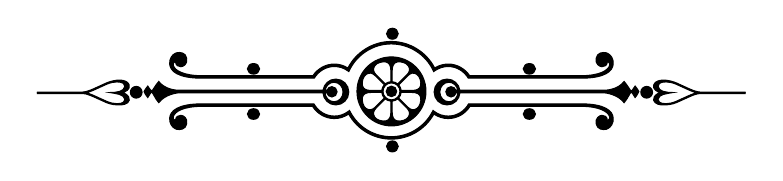
\begin{tikzpicture}
    \node  (C) at (0,0) {};
    \node (D) at (9,0) {};
    \path (C) to [ornament=84] (D);
    \end{tikzpicture}}}}}%
    \end{center}
  }
  
\newcommand{\EnglischeLinie}{
\sectionline{darkRed!60!cyan}
}

\newcommand{\whEnglischeLinie}{
\sectionline{white}
}
% ///


\newcommand{\sectionlinenoc}[2]{%
	\noindent
		{\color{#1}
			\resizebox{#2}{1ex}
			{{%
					{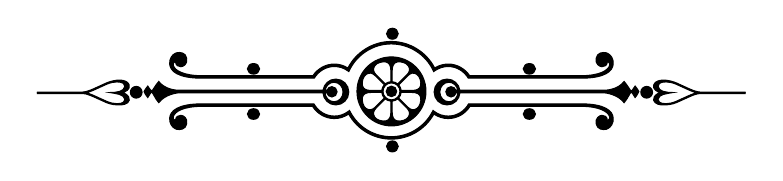
\begin{tikzpicture}
						\node  (C) at (0,0) {};
						\node (D) at (9,0) {};
						\path (C) to [ornament=84] (D);
						\end{tikzpicture}}}}}%
}

\newcommand{\shortsectionline}[1]{%
	\noindent
	\begin{center}
		{\color{#1}
			\resizebox{.2\linewidth}{1.5ex}
			{{%
					{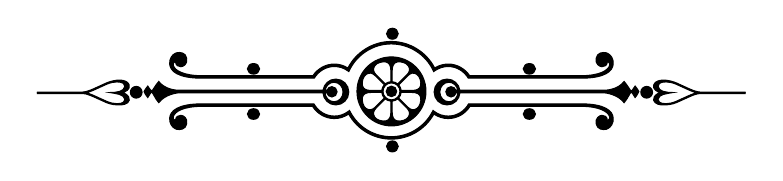
\begin{tikzpicture}
						\node  (C) at (0,0) {};
						\node (D) at (9,0) {};
						\path (C) to [ornament=84] (D);
						\end{tikzpicture}}}}}%
	\end{center}
}

\definecolor{blGreen}{rgb}{.2,.7,.3}

\newcommand{\shortdecoline}{\vspace*{-.65em}\shortsectionline{blGreen!10!orange}\vspace*{-.85em}}
\newcommand{\shortdecolineadj}[2]{\vspace*{#1}\shortsectionline{blGreen!10!orange}\vspace*{#2}}


\usepackage[flushmargin]{footmisc}

\usepackage[letterpaper, left=.45in,right=.45in,top=1in,bottom=1in]{geometry}

\colorlet{codegr}{black!80!blue}

\setlength{\columnsep}{7mm}

%% rightx
\newcommand{\htwoo}{H$_2$O}
\newcommand{\dtwoo}{D$_2$O}
\newcommand{\POne}{$P_1$}
\newcommand{\PTwo}{$P_2$}
\newcommand{\Pone}{$P_1$}
\newcommand{\Ptwo}{$P_2$}
\newcommand{\Pprop}{$P$}

\newcommand{\Stwo}{$S_2$}
\newcommand{\Sone}{$S_1$}

\newcommand{\facondeparler}{\textit{fa{\c{c}}on de parler}}

\newcounter{sentenceCounter}{}

\newcommand{\writeIncSentenceCounter}{\refstepcounter{sentenceCounter}(\arabic{sentenceCounter})}{}


\newcommand{\listItemMark}{\rotatebox{30}{\raisebox{2pt}{\color{green!30!yellow!40!black}{\begin{tiny}$\blacktriangleright$\end{tiny}}}}}
\newenvironment{sentenceList}{\begin{list}{\listItemMark}{\setlength{\leftmargin}{.5em}\setlength{\itemsep}{-.1em}\setlength{\topsep}{.85em}}\begin{small}}{\end{small}\end{list}}

\newcommand{\sentenceItem}{\item \writeIncSentenceCounter}{}
% ///

\usepackage{etoolbox}

\AtBeginEnvironment{thebibliography}{\linespread{1}\selectfont}

%?\usepackage{mathptmx}


%?\titleformat*{\subsection}{\small\bfseries}

%?\usepackage{eufrak}
\usepackage{wasysym}
\usepackage{textcomp}
\usepackage{amssymb}

\usepackage{microtype}



\DeclareMathAlphabet{\mathcal}{OMS}{cmsy}{m}{n}
%\usepackage{euler}

\let\OldI\i


\newcommand{\mdash}{---}
\newcommand{\q}[1]{``#1"}
\newcommand{\sq}[1]{`#1'}
\renewcommand{\i}[1]{\textit{#1}}

\newcommand{\T}[1]{\raisebox{-2pt}{\ensuremath{\mathcal{T}}}\textit{\tiny #1}}
%\newcommand{\T}{\ensuremath{\mathscr{T2}}}

\newcommand{\TSupT}{\ensuremath{{\T2}\makebox[4pt][r]{\raisebox{5pt}{{\scalebox{.6}{\T1}}}}}}

\let\OldFootnoteSize\footnotesize
\renewcommand{\footnotesize}{\scriptsize}
	
%\newcommand{\Tnoindex}{\raisebox{-2pt}{\ensuremath{\mathfrak{t}}}}
\newcommand{\Tnoindex}{\ensuremath{\mathfrak{t}}}

\newcommand{\typeAbove}{%
\raisebox{-1pt}{\rotatebox{90}{\begin{tiny}$\diagdown$\makebox[1pt][c]{$\diagup$}\end{tiny}}}}

%\newcommand{\typeT}{\ensuremath{type\raisebox{.5pt}{\makebox[3pt][c]{-}}T}}
%\newcommand{\typeT}{\ensuremath{\mathcal{T}}}
\newcommand{\typeT}{\ensuremath{\mathfrak{t}}}

\newcommand{\TValues}{\typeT{}-values} 

\newcommand{\emigres}{\'emigr\'es}

\newcommand{\Retore}{Retor\'e}
\newcommand{\Aurelie}{Aur\'elie}
\newcommand{\Descles}{D\'escles}

\newcommand{\ala}{\`a la}

\newcommand{\picalculus}{\ensuremath{\pi}-calculus}

\newcommand{\qmarkdubious}{\raisebox{4pt}{{\footnotesize\textbf{?}}}}

%\newcommand{\TypeCat}{\ensuremath{\mathcal{T}}}
\newcommand{\TypeCat}{\ensuremath{\mathfrak{t}}}

\newcommand{\ADJplusNPeqNP}{\ensuremath{ADJ + NP = NP}}

%\newcommand{\outarrow}{\ensuremath{\overset{..}{\rightarrow}}}

\newcommand{\outarrow}{\makebox[-2pt][l]{%
\raisebox{4pt}{..}}\ensuremath{\rightarrow}}

\newcommand{\argarrow}{\hspace{1pt} \makebox[-2pt][l]{%
		\raisebox{4pt}{.}}\ensuremath{\rightarrow} \hspace{1pt}}


\newcommand{\smoutarrow}{\makebox[-1pt][l]{%
		\raisebox{3pt}{..}}\ensuremath{\rightarrow}}

\newcommand{\smargarrow}{\hspace{1pt} \makebox[-2pt][l]{%
		\raisebox{3pt}{.}}\ensuremath{\rightarrow} \hspace{1pt}}



%\newcommand{\NounToNoun}{N \outarrow N}
%\newcommand{\VisNtoS}{V :: N \outarrow N}

\newcommand{\mmbox}[1]{#1}

\newcommand{\NtoN}{\mmbox{\ensuremath{N} \outarrow{} \ensuremath{N}}}
\newcommand{\NounToNoun}{\mmbox{\ensuremath{N} \outarrow{} \ensuremath{N}}}
\newcommand{\VisNtoS}{\mmbox{\ensuremath{V :: N} \outarrow{} \Prop}}
\newcommand{\AdjisNtoN}{\mmbox{\hspace{2pt}\ensuremath{\mathcal{A}
\scalebox{.7}{\ensuremath{\mathcal{DJ}}} :: N} \outarrow{} \Prop}}


\newcommand{\thatPhrase}{\AcronymText{that}-phrase}
\newcommand{\thatPhrases}{\AcronymText{that}-phrases}

\usepackage{graphicx}

\newcommand{\rzauthor}[3]{{
{\vspace{-4em}}{\fontfamily{gar}\fontseries{b}\selectfont% 
{\begin{center}\textls*[103]{#1}\\ \vspace{-2em}%
{\scalebox{.7}{\fontfamily{phv}\fontshape{it}\selectfont\footnotesize #3}}#2\end{center}}

{\vspace{-2.25em}}
{\hfill\small\today}

{\vspace{.25em}}
}}}			 


\newcommand{\rzauth}[3]{{
		{\vspace{-1em}}{\fontfamily{gar}\fontseries{b}\selectfont% 
			{\begin{center}\textls*[103]{#1}\\ \vspace{1em}%
					{\scalebox{.7}{\fontfamily{phv}\fontshape{it}\selectfont\footnotesize #3}}#2\end{center}}
			
			{\vspace{-6em}}
			{\hfill\small {\raisebox{1em}{\today}}}
			
			{\vspace{0em}}
		}}}			 




\newcommand{\rztitle}[1]{\begin{center}\fontfamily{phv}\fontseries{b}\selectfont #1\end{center}}


\newcommand{\Jorgen}{J{\o}rgen}

\newcommand{\Prop}{\ensuremath{\mathcal{P}rop}}

\newcommand{\NN}{\ensuremath{N}\hspace{-1pt}\argarrow\hspace{-1pt}\ensuremath{N}}
\newcommand{\Npl}{%
\ensuremath{N}\raisebox{8pt}{\hspace{-1pt}\ensuremath{\rotatebox{180}{{\begin{footnotesize}$\dotplus$\end{footnotesize}}}}}}
\newcommand{\NPl}{\Npl}
\newcommand{\NtoNpl}{%
\mmbox{\ensuremath{N} \outarrow{} \Npl}}
\newcommand{\NpltoNpl}{\mmbox{\Npl{} \outarrow{} \Npl}}
\newcommand{\PropToN}{\mmbox{\Prop \hspace{1pt} \outarrow{} \N}}

\newcommand{\VisNNtoProp}{\mmbox{\ensuremath{V :: N} \argarrow \ensuremath{N} \outarrow{} \Prop}}
\newcommand{\VisNProptoProp}{\mmbox{\ensuremath{V :: N} \argarrow  \Prop{} \hspace{2pt} \outarrow{} \Prop}}


\newcommand{\NSing}{\ensuremath{N}\raisebox{5pt}{\scalebox{0.65}{\ensuremath{%
{\odot}}}}}


\newcommand{\Z}{\ensuremath{\mathbb{Z}}}

\newcommand{\VPpNPeqS}{\ensuremath{VP + NP = S}}
\newcommand{\NSingToNPl}{\mmbox{\NSing{} \outarrow{} \Npl}}

\newcommand{\NNtoS}{\mmbox{\NN{} \outarrow{} \Prop}}
\newcommand{\NNtoN}{\mmbox{\NN{} \outarrow{} \ensuremath{N}}}
\newcommand{\N}{\mmbox{\ensuremath{N}}}
\newcommand{\NtoProp}{\mmbox{\N{} \outarrow{} \Prop}}
\newcommand{\NNtoProp}{\mmbox{\NN{} \outarrow{} \Prop{}}}
\newcommand{\ProptoN}{\mmbox{\Prop{} \outarrow{} \N}}


\newcommand{\PropToNYieldsN}{\PropToN{} \raisebox{1pt}{\ensuremath{\textgreater\hspace{-5pt}\raisebox{.15pt}{\ensuremath{\Rightarrow}}}}{} \N}

\newcommand{\SeqNPplVP}{\mmbox{{\small\texttt{S = NP + VP}}}}

\newcommand{\Arg}{\ensuremath{A}\tiny{rg}}
\newcommand{\argsToReturn}{\mbox{\ensuremath{{\Arg}_0} \hspace{-4pt} \smargarrow 
		\hspace{-3pt}
\ensuremath{{\Arg}_1} 
\hspace{-4pt} \smargarrow \hspace{-2pt} \ensuremath{\cdot\cdot\cdot} \hspace{0pt} \smoutarrow  \hspace{1pt} \textit{Result}}}

\newcommand{\lowBlank}{\raisebox{-1pt}{\textthreequartersemdash\textthreequartersemdash\textthreequartersemdash}}

\newcommand{\BlankAfterBlank}{\lowBlank\texttt{after}\lowBlank}
\newcommand{\AfterNSingAndNSingToNPl}{\mbox{\texttt{after} :: %
\NSing \argarrow \NSing \hspace{1pt} \outarrow \hspace{1pt} \Npl}}

\newcommand{\archiveDate}[1]{{\footnotesize #1}}

\newcommand{\sentenceexample}[1]{
\begin{noindent}
\hspace*{-8pt}{{\raisebox{2pt}{{\scriptsize {\color{green!30!yellow!40!black}  
\rotatebox{20}{\RIGHTarrow}}}}} \hspace*{-2pt} #1
	
}
\end{noindent}
}

\newcommand{\sentenceexamples}[1]{
	
\vspace{1em}		
{\setstretch{1.0}	
#1
}
\vspace{.7em}		

\noindent\hspace{-4pt}}



\newcommand{\FeqMtimesA}{\hspace{-2pt}{\small \ensuremath{F}=\ensuremath{M}{\texttimes}\ensuremath{A}}}
\newcommand{\piCalculus}{\ensuremath{\pi}-calculus}


\newif\iffootnote
\let\Footnote\footnote
\renewcommand\footnote[1]{\begingroup\footnotetrue\Footnote{#1}\endgroup}

\newcommand{\AcronymText}[1]{{\iffootnote\begin{footnotesize}{\textsc{#1}}\end{footnotesize}%
\else\begin{OldFootnoteSize}{\textsc{#1}}\end{OldFootnoteSize}\fi}}


\newcommand{\NLP}{\AcronymText{NLP}}
\newcommand{\POS}{\AcronymText{POS}}

\newcommand{\Gardenfors}{G\"ardenfors}


\newcommand{\Haskell}{\AcronymText{Haskell}}
\newcommand{\C}{\AcronymText{C}}
\newcommand{\NP}{\AcronymText{NP}}
\newcommand{\Cpp}{\AcronymText{C++}}
\newcommand{\RDF}{\AcronymText{RDF}}
\newcommand{\Java}{\AcronymText{Java}}
\newcommand{\IT}{\AcronymText{IT}}
\newcommand{\IBMinc}{\AcronymText{IBM}}
\newcommand{\XDG}{\AcronymText{XDG}}
\newcommand{\AI}{\AcronymText{AI}}

\newcommand{\HPSG}{\AcronymText{HPSG}}
\newcommand{\CAG}{\AcronymText{CAG}}
\newcommand{\Lisp}{\AcronymText{Lisp}}

\newcommand{\TS}{\AcronymText{TS}}

\newcommand{\ThreeD}{\AcronymText{3D}}

%?\usepackage[inline]{enumitem}
\usepackage{enumitem}




\usepackage[font=small,labelfont=bf]{caption}

\usepackage{xcolor}

\definecolor{Bkg}{RGB}{250,245,252}
\newcommand{\leader}[2]{\hspace{#1}\colorbox{Bkg}{#2}}


\newcommand{\saying}[1]{\vspace{2ex}\noindent{%%
				\leader{2em}{\begin{minipage}{.38\textwidth}{\footnotesize #1}\end{minipage}}\vspace{2ex}}}

\newcommand{\sayingsrc}[1]{\vspace{0ex}\\\hspace{2pt} --- {\footnotesize #1}}

\renewcommand{\labelitemi}{$\blacklozenge$}

\newcommand{\itemmark}{\raisebox{-4pt}{\rotatebox{90}{{\Large $\bracevert$}}}}

\usepackage{tikz}
\usetikzlibrary{positioning}
\usetikzlibrary{shapes,snakes}

\newcommand{\visavis}{vis-\`a-vis}

%\sectionfont{\fontsize{12}{8}\selectfont}


\newcommand{\underlines}{{\normalsize \lowBlank\hspace{.1em}}}
%\newcommand{\underlines}{{\normalsize \lowBlank\lowBlank\lowBlank\hspace{.5em}}}

\newcommand{\XAcrossY}{\mbox{\ensuremath{x} \texttt{across} \ensuremath{y}}}

\newcommand{\Rel}{\raisebox{.5pt}{\texttt{{\OldFootnoteSize r}}}}

\newcommand{\XRelY}{\mbox{\ensuremath{x} \Rel{} \ensuremath{y}}}

\newcommand{\tinyurl}[1]{{\raisebox{2pt}{{\scriptsize \url{#1}}}}} 

\usepackage[colorlinks=true]{hyperref}

\colorlet{urlclr}{red!40!magenta!50!orange}

\hypersetup{
 urlcolor = urlclr,
 urlbordercolor = cyan!60!black,
 linkcolor = red!30!black,
 citecolor = orange!30!black,
 citebordercolor = yellow!30!black,
} 


\makeatletter
\Hy@AtBeginDocument{%
	\def\@pdfborder{0 0 0}% Overrides border definition set with colorlinks=true
	\def\@pdfborderstyle{/S/U/W .25}% Overrides border style set with colorlinks=true
	% Hyperlink border style will be underline of width 1pt
}
\makeatother


%\titlespacing{\section}{.25\textwidth}{*2.8}{*-.4}[5pc]


\newcommand{\p}[1]{
	
	\vspace{.575em}
	#1	
}

\renewenvironment{abstract}
{\small
	\begin{center}
		\bfseries \abstractname\vspace{-.5em}\vspace{0pt}
	\end{center}
	\list{}{%
		\setlength{\leftmargin}{.43in}% <---------- CHANGE HERE
		\setlength{\rightmargin}{\leftmargin}%
	}%
	\item\relax}
{\endlist}


\let\OldSection\section
\renewcommand\section[1]{
	\vspace{5pt}
	\OldSection{#1}
	\vspace{-4pt}
}

%?\let\OldSubsection\subsection

%?\renewcommand\subsection[1]{
%?	\vspace{-5pt}
%?	\OldSubsection{#1}
%?	\vspace{-16pt}
%?}

\usepackage{transparent}

\definecolor{logoCyan}{RGB}{66, 206, 244}
\definecolor{logoBlue}{RGB}{4, 2, 25}

\titleformat*{\subsection}{\Large\bfseries}

\let\OldSubsection\subsection
\renewcommand\subsection[1]{

	\vspace{12pt}
	
    %{\LARGE
	%\colorbox{logoCyan}{%
	%\begin{minipage}{\linewidth}
		\OldSubsection{% 	
			\hspace{-2.75em}
			%\begin{minipage}{}
			\protect\raisebox{-5pt}{%
			\colorbox{logoCyan!50}{\hspace{2.1em}}}%
			\hspace{-5pt}{\protect\transparent{0.3}{\colorbox{logoBlue!80}{\protect\transparent{1}{%
						   \protect\raisebox{1pt}{\textit{{\large #1}}} }}}}
			%\end{minipage}
		}
	%\end{minipage}
    %}
    %}
	\vspace{-6pt}
}


\newsavebox{\twolinebox}

\newcommand{\stwoline}[1]{%
\sbox{\twolinebox}{\raisebox{-3pt}%
{\parbox{7.4cm}{\linespread{1.25}\selectfont\raggedleft{\textit{\textbf{{\large #1}}}}}}}}

\newcommand{\twoline}{\usebox{\twolinebox}}

\newcommand{\subsectiontwoline}[1]{\stwoline{#1}\subsection{\twoline}}

\newcommand{\spsubsection}[1]{%
\vspace{-.25em}
\subsection{#1}
\vspace{.3em}
}
\newcommand{\spsubsectiontwoline}[1]{%
\subsectiontwoline{#1}
\vspace{.3em}
}




\let\OLDthebibliography\thebibliography
\renewcommand\thebibliography[1]{
\let\section\OldSection
\setlength{\leftmargin}{-4pt}
\vspace{.1em}
\OLDthebibliography{#1}
\vspace{.7em}
\OldFootnoteSize 
\setlength{\parskip}{0pt}
\setlength{\itemsep}{2.3pt plus 0ex}
\raggedright
}

\makeatletter
%\def\@biblabel#1{\hspace{-6pt}[#1]}
\def\@biblabel#1{\hspace{-6pt}#1}
\makeatother

\newcommand{\bibtitle}[1]{{\small \textit{#1}}}
\newcommand{\intitle}[1]{{\hspace{3pt}\textls*[-80]{\texttt{\textit{#1}}}}\hspace{-1pt}}

\renewcommand{\i}[1]{\textit{#1}}




\newcommand{\itemtitle}[1]{{\color{green!10!red!40!black} \textls*[-80]{\texttt{#1}}}}
\newcommand{\MIT}{\AcronymText{MIT}}

\newcommand{\nulltt}{\AcronymText{\texttt{null}}}
\newcommand{\Maybe}{\AcronymText{\texttt{Maybe}}}
\newcommand{\bind}{\AcronymText{\texttt{bind}}}
\newcommand{\return}{\AcronymText{\texttt{return}}}

\newcommand{\XML}{\AcronymText{XML}}
\newcommand{\XQuery}{\AcronymText{XQuery}}
\newcommand{\XQueries}{\AcronymText{XQueries}}
\newcommand{\API}{\AcronymText{API}}
\newcommand{\IR}{\AcronymText{IR}}
\newcommand{\Clang}{\AcronymText{Clang}}
\newcommand{\DAG}{\AcronymText{DAG}}
\newcommand{\DAGs}{\AcronymText{DAG}s}

\newcommand{\Qt}{\AcronymText{Qt}}
\newcommand{\NL}{\AcronymText{NL}}
\newcommand{\langC}{\AcronymText{C}}
\newcommand{\SDK}{\AcronymText{SDK}}

\newcommand{\SOV}{\AcronymText{SOV}}
\newcommand{\SVO}{\AcronymText{SVO}}

\newcommand{\YtwoK}{\AcronymText{Y2K}}

\newcommand{\qi}[1]{\q{\textit{#1}}}

\newcommand{\CSharp}{\AcronymText{C\#}}

\newcommand{\Tesniere}{Tesni\`ere}

\newcommand{\sentenceExample}[1]{``#1"}


\newcommand{\expose}{expos\'e}
\newcommand{\ExistsX}{\ensuremath{{\exists}X:Hugo(X){\wedge}Cat(X)%
{\wedge}Sleeps(X,on-the-couch)}}
\newcommand{\Exists}{\ensuremath{\exists}}
\newcommand{\ndim}{\ensuremath{n}-dimensional}

\usetikzlibrary{decorations.pathmorphing}

\newcommand{\longdash}{---}

\usepackage[breakable]{tcolorbox}% http://ctan.org/pkg/tcolorbox

\newenvironment{frquote}{%
%\begin{fcolorbox}{yellow!20!gray}{red!5}
%\begin{flushright}
\begin{tcolorbox}[
	colback=orange!6,
	colframe=yellow!20!gray,
	width=1.95\linewidth,
	arc=3mm, auto outer arc
	]
\begin{scriptsize}
\begin{minipage}{57em}
\begin{flushright}
\begin{minipage}{58em}}{%
\end{minipage}
\end{flushright}
\end{minipage}
\end{scriptsize}
\end{tcolorbox}
%\end{flushright}
}

\newcommand{\kErn}{\ensuremath{\mathcal{K}}}
\newcommand{\tSys}{\ensuremath{\mathbb{T}}}

%\newcommand{\tSys}{\ensuremath{T}}

\newcommand{\procOne}{\ensuremath{\mathcal{P}_1}}
\newcommand{\procTwo}{\ensuremath{\mathcal{P}_2}}
\newcommand{\fFunT}{\ensuremath{\mathcal{F}_t}}
\newcommand{\ChaOne}{\ensuremath{\mathcal{C}_1}}
\newcommand{\ChaTwo}{\ensuremath{\mathcal{C}_2}}
\newcommand{\CarOne}{\ensuremath{\mathfrak{c}_1}}
\newcommand{\CarTwo}{\ensuremath{\mathfrak{c}_2}}
\newcommand{\CarHandoffCar}{\ensuremath{\mathfrak{c}_1{\looparrowright}\mathfrak{c}_2}}
\newcommand{\ChpAlliedChx}{\ensuremath{\mathcal{C}_p{\circledcirc}\mathcal{C}_x}}
\newcommand{\Chp}{\ensuremath{\mathcal{C}_p}}
\newcommand{\Chx}{\ensuremath{\mathcal{C}_x}}
\newcommand{\ChaProductCha}{\ensuremath{\mathcal{C}_1{\otimes}\mathcal{C}_2}}

\newcommand{\stageLbl}{\ensuremath{\mathcal{L}}}
\newcommand{\DigammaR}{\ensuremath{{\varsigma}{\pointer}{\stageLbl}}}

\newcommand{\sigmaCalc}{\ensuremath{\varsigma} Calculus}
\newcommand{\voidP}{void*}
\newcommand{\ChaAppendCar}{\ensuremath{\mathcal{C}{\oplus}\mathfrak{c}}}
\newcommand{\LappendX}{\ensuremath{\mathcal{L}{\ll}\mathcal{X}}}
\newcommand{\Lprime}{\ensuremath{\mathcal{L}'}}
\newcommand{\LpreX}{\ensuremath{\mathcal{L}}}
\newcommand{\tTyp}{\ensuremath{\mathfrak{t}}}
\newcommand{\xy}{\ensuremath{xy}}



\AddToShipoutPicture{%
  \AtPageLowerLeft{%
    \hspace*{1em}
 \rotatebox{90}{%
        \begin{minipage}{\paperheight}
   \centering
   {\color{codegr!65}\textcopyright ~\today{} Nathaniel Christen}
        \end{minipage} %
      }
    } %
  }%
\begin{document}\title{Hypergraph Data Modeling and a Hypergraph Virtual Machine}
\maketitle{}
\begin{abstract}This paper will argue for multi-purpose hypegraph data models as a 
generic representation paradigm for data sharing and publication.  
Seeking to unify disparate constructions where hypergraphs generalize 
ordinary (labelled, directed) graphs, I propose a multi-disciplinary 
hypergraph framework which captures hypergraph structures found 
in mathematics, linguistics, computer science, and related disciplines.  
I consider how to integrate these varying structures and propose an 
overarching generalized model which I call \q{procedural} hypergraphs 
and a \q{Procedural Hypergraph Ontology} (Phaon).    
I then discuss hypergraph representations of computer code and 
implementation strategies for a runtime execution environment 
with hypergraphs as the principle internal data representation.  
This paper is paired with a code repository demonstrating such a 
Hypergraph Virtual Machine (Phaon Virtual Machine, or \PVM{}).  
I outline parsing and compiler techniques for \PVM{} as a 
case-study in the supporting ecosystem necessary for 
hypergraph paradigms to be useful in lieu of, for 
instance, Semantic Web Ontologies.
\end{abstract}
\begin{frquote}On conna\^{\OldI}t la c\'{e}l\`{e}bre affirmation de Claude L\'{e}vi-Strauss: 
\q{les sciences humaines seront structurales ou ne seront pas}.  Nous aimerions lui en
adjoindre une autre: \q{les sciences humaines seront des sciences naturelles ou ne seront pas}. 
Evidemment, sauf \`{a} en revenir \`{a} un r\'{e}ductionnisme dogmatique, une telle
affirmation n'est soutenable que si l'on peut suffisamment g\'{e}n\'{e}raliser le concept
classique de \q{naturalit\'{e}}, le g\'{e}n\'{e}raliser jusqu'\`{a} pouvoir y faire droit, 
comme \`{a} des ph\'{e}nom\`{e}nes naturels, aux ph\'{e}nom\`{e}nes d'organisation structurale.
\\ \longdash{} Jean Petitot, \cite[p. 1]{PetitotSyntaxe}{}
\end{frquote}
\begin{frquote}What does $M$ really do in the information system?  It acts as
an interface between the (external) world and the control 
system.  It structures influences to allow focused purposeful
control.  If any sense of significance can be given
to a particular state $m$ of $M$, it must be related
to this interface function.  The
significance of $m$ is neither that it
tracks something external nor
that it can affect the
control mechanisms of the system,
but that it can connect one to the
other.  The idea of interface allows
us to specify a notion of meaning for a datum
in an information system ... in the whole process
of purposeful interaction between the information system and the environment.
\\ \longdash{} Orlin Vakarelov, \cite[p. 15-16]{OrlinVakarelov}{}
\end{frquote}
\vspace{1em}
\p{Computational and scientific data representation intrinsically 
balances two competing priorities: \q{semantic} expressiveness and 
computational tractability.  On the one hand, representations should not 
obscure important details: the formal requirements on 
representational validity should not force representations 
into structures that necessitate the elimination of meaningful 
information.  On the other hand, conversely, representations 
should have enough structural consistency that they are 
amenable to analysis and transformations driven by 
formal algorithms.
}
\p{I have just left a lot of loose ends: in particular, these comments need 
to give some meaningful definition to \q{representation}.  There 
are many media wherein \q{data} can be represented: via graphics 
(e.g., charts, \q{maps} in the cartographical sense, or \q{graphs} 
in the sense of plotted visualizations of 
mathematical functions), via printed documents (like the logarithmic 
tables or astronomic records of early modern science), or via mathematical 
equations and formulae (if a mathematical theory correctly 
predicts and quantifies empirical data \mdash{} e.g., fitting trajectories 
to elliptic or parabolic shapes \mdash{} then the numeric structures of 
the theory are a proxy representation of the corresponding data).  
Moreover, aside from these relatively formal modes of representation, 
we have the capacity to indirectly describe information via 
natural language. 
}
\p{The modern age has a further notion of representation: \i{digital} 
representations which leverage the capabilities of 
computer storage and processing to create persistent 
data repositories, with the possibility of manipulating 
data via computer programming and displaying data 
via computer software.  These digital representations incorporate 
features of the older representational media I alluded to: 
like Natural Language digital data often emanates from a 
textual representation, with data structures initialized 
from special \q{languages} like \XML{} or \JSON{}.  As with 
structured \q{printed} documents (of the astronomical-table 
or even grocery-shopping-list variety), digital representations 
often build off of a rigid structural template, like a two-dimensional 
table with rows and columns, or a hierarchical document 
whose elements can be nested documents.  And as with 
mathematical representations, digital representations can be 
analyzed as instances of spaces or structures with certain 
algebraic or syntactic properties and requirements.  
It is often possible to mathematically describe the 
full space of structures which conform to a given 
representational protocol, or the full space of transformations 
that can modify a given data structure while staying 
consistent with its enforced protocols.  Also, each data 
structure potentially has some notion of aggregateness: of 
having different \q{parts}, of being able to focus on one part 
at a time, and to \q{move} focus from one part to another.  
Given these qualities, digital representations extend and integrate 
the affordances of print, graphical, and linguistic media 
\mdash{} but they do so in an electronic environment that permits digital 
archives to be accessed via computer software.   Given this access, 
digital representations can inherit the formal properties of the software 
that uses them, so we can think of digital representations as formal 
structures themselves, amenable to something like a mathematical analysis. 
}
\p{In short, digital representations have several general criteria: 
\i{validity} (a formal model of conformant vs. invalid 
structures\footnote{An invalid graph might be a case where an 
edge has no incident nodes; an invalid \XML{} structure is one without 
a single root element or (insofar as such a structure would be 
representable) with mismatched tags, and so forth)}); 
\i{traversability} (a notion of parthood and iterating
or refocusing among parts), and, let's say, \i{atomicity} 
(a notion of unitary parts that can be represented as 
integral wholes).  These criteria ensure that digitally 
represented data structures can work within software and 
networking representations: information is 
presented to software users by displaying atomic 
units (textually or graphically) and traversing through 
data structures to fill in, via application code, a 
visual tableau presenting compound data, with different 
unitary displays visually separated and often organized into 
coherent visual patterns, like the grid-pattern of a 
spreadsheet.  Meanwhile, atomic units can be textually 
encoded, and aggregate structure likewise notated through 
syntactic conventions that preserve atom's boundaries, yielding 
textual serializations of data structures that can be 
shared between computing environments, allowing information to 
be copied and distributed.  Finally, digital representations 
of data structures canbe marshalled into different binary forms \mdash{} 
encoded in byte- and bit-patterns \mdash{} to enable both 
persistent storage in a database and \q{runtime} presence 
as binary data that can be accessed by software applications.
}
\p{I take the time to lay out these basic principles because I want 
to emphasize the different contexts where digital representations can be 
found: in particular, textual encoding and serialization; 
graphical/interactive displays for software users; application runtimes; 
and long-term database storage.  A given representation will morph and 
mutate to accommodate these different contexts.  Moreover, these 
contexts correspond to distinct technical specializations: database engineers 
have a different perspective on data structures than network engineers designing 
protocols for encoding and exchanging data between network endpoints; and 
application designers focused on optimal human-computer-application 
understand digital representations as visual and interactive phenomena, 
whereas application \i{developers} need to focus on how to 
properly encode data structures for binary runtimes.  These various 
perspectives all influence the theory and technology 
behind digital data representation: a successful 
representational paradigm needs to adapt to the operatoonal 
requirements of engineers in each of these disicplines.
}
\p{Additionally, insofar as the point of digital archives is to encode 
empirical, \q{real-world} data, a proper representational protocol 
needs to promote a synergy between the information as humans understand 
it and the data structures recognized bu the technology.  For instance, 
if a published data set shares scientific data, it should be 
represented in ways that preserve scintifically significant 
details \mdash{} any derivations, descriptions, or observations 
which are intrinsic to the science's methodology, 
theory, assumptions, and experimental results.  The data needs to 
be structured according to the \q{semantics of the science}, so that 
the scientific background can be reconstructed along with future use 
of the data, even after a circuitous journey through different 
contexts, like through a database and over a network to 
a scientific-software application (maye years later).   
As formal models of data semantics have become more rigorous \mdash{} e.g. in our 
century with Ontologies and the \q{Semantic Web} \mdash{} this 
\q{semantic engineering} has become a further technical perspective 
needing consideration in the dsign and evaluation of digital representations.
}
\p{Over the decades, many general representation strategies and 
\q{layouts} have been envisioned, from tabular structures 
in the manner of Relational Databases, to tree-like 
documents whose morphology is inspired by markup languags, 
to structurally looser variations on row/column 
arrangements like multi-dimensional key-value spaces or 
\q{Big Column} and other \q{\NoSQL{}}-database-inspired 
articulations.  These various paradigms are subject to 
\q{selective} pressures based on how well the meet the 
different engineering needs I have identified.  But the 
multiplicity of these needs complicates the \q{competition} between 
representational strategies: a paradigm optimized 
for one context (e.g., persistent databases) is not necessarily 
optiman for another (e.g., application and \GUI{} development).  
As a result, developers and computer scientists must 
continue to explore and collaborate on new paradigms which 
work better across contexts.
}
\p{In the plurality of representational paradigms, a significant 
evolution has been the emergent popularity of structures 
based on graphs.  The predominant influence on this 
line of development has been the Semantic Web and the specific graph 
architecture codified by \q{Web Ontologies}, although 
other graph-representation models (such as 
Conceptual Graph Semantics) were also candidates for 
potential technological \q{entrenchnment} before 
Semantic Web formats like \RDF{} and \OWL{} 
became standardized.\footnote{Why \RDF{}/\OWL{} and not, say, Conceptual 
Graphs, or the hybrid Object-Database/Graph-Database models 
studied in the 1990s, became canonized in the Semantic Web, is 
an interesting question but perhaps of mostly historical 
interest insofar as Hypergaphs can unify each of these paradigms.
}  More recently, scientists have proposed generalizations 
and/or alternatives to the Semantic Web based on 
hypergraphs in lieu of ordinary (directed, labeled) graphs.
}
\p{As might be ascertained from hypergraphs being the focus of this paper, 
I believe that representational paradigms based on hypergraphs can be superior to 
other formats and need to be studied with an integrated, generalized 
set of theories and computer tools.  I have inrododucd the 
topic of hypergraph data structures via the general issues in 
digital representation in part to rest claims of hypergraphs' 
merit on explicit criteria.  In particular, I believe 
hypergraphs can adapt to the different technological 
contexts prerequisute to a decentralized digital ecosystem 
\mdash{} databases, networking, application implementation, visual/interactive 
software design, and semantic expressiveness \mdash{} more effeectively 
than other paradigms, like regular graphs or \SQL{}-style tables.  
I suspect other scientists and engineers have 
similar intuitions, because there has been a recent uptick in 
research on hypergraphs in various disciplines, such 
as Category Theory, Information Management, Artificial Intelligence, 
and Natural Language Processing.  Compared to 
the Semantic Web, however, there is a noticeable lack 
of standard tools or formats for expressing hypergraph 
data or sharing hypergraph structures across multiple 
applications and environments.  Where \RDF{} and \OWL{} are 
definitely associated with the Semantic Web, so that 
supporting these standards is a basic entry point for 
Semantic Web technologies, there is no comparable 
consensus on the underlying theory of hypergraph data 
in general.    
}
\p{This situation may be explained in part by subtle differences on 
what the word \q{hypergraph} is supposed to mean in different 
settings, so the overal terrain of hypergraphs is 
divided into distinct mathematical models, often without a 
rigorous theory of their interrelationships.  
Another problem is perhaps a failure to appreciate how hypergraphs 
are structurally different from ordinary graphs, so that 
hypergraph-shaped data may be imprecisely treated as 
a mere variation upon or a special structuration within 
ordinary graphs.  For eample, Semantic Web structures such as 
\RDF{} \q{bags} and \q{collections} introduce a kind of 
hierarchical organization to Semantic Web graphs, and can be considered 
a form of hypergraph, but these protocols are not described as 
enabling a transition from a networking framework based on 
directed labeled graphs to one based on hypergraphs.  Instead, 
hypergraphs become \i{de facto} embedded within ordinary graphs, 
exploiting the representational flexibility which also 
makes the Semantic Web suitable for spreadsheets, \XML{}, and 
other structures that are not graphs at a \i{prima facie} level.
The problem is that while hypergraphs can be \i{encoded} in 
ordinary graphs with a suitable labeling convention, 
the distinct structural details which make hypergraphs 
superior to the Semantic Web no longer remain as 
explicit architectural features once hypergraphs are 
\q{encoded} in conventional Semantic Web formats.
}
\p{Recent (computer-science-related) research into hypergraphs 
sems to emphasize two different topics: first, the 
representational potential for hypergraphs as a 
general morphology for representing structured information 
in general; and, second, the specific possibilities 
of using hypergraphs to model computer code and computational 
processes.  In the second subject-area, hypergraphs are studied 
as a medium for expressing details about computer algorithms as a 
way to reason about executable computer code as a structured system, and 
perhaps even design execution engines (virtual machines to 
run computer code that is in a suitable representation).  This 
latter research sometimes appears to present a mathematical 
picture of hypergraphs as an abstract model 
of computing procedures and evaluations \mdash{} a kind of 
graph-based rinterpretation of the lambda calculus \mdash{} but 
sometimes is also marshaled into implemented execution 
environments, as in the OpenCog and lmnTal frameworks.
}
\p{My goal in this paper is to consider what a unified hypergraph 
paradigm can look like \mdash{} how the different strands which in their 
own way embody hypergraph structures can be woven together 
into a multi-purpose whole.  My emphasis is on computer implementations 
rather than mathematics \mdash{} that is, I will not present axioms 
or theorems formalizing different sorts of hypergraphs, though I 
ackowledge that such descriptions are possible.  Instead, my 
aim is to describe what might constitute a general software 
library or toolkit that can adapt to different hypergraph 
models and use-cases.  This paper is accompanied by a \q{data set} 
which involves a library (written in \Cpp{}) for creating and 
manipulating hypergraphs of different varieties, and also a 
\q{virtual machine} for modeling and realizing 
computatational procedures via hypergraph structures.  The 
point of the accompanying code is to 
demonstrate that a generalized hypergraph representation 
is possible, and that in addition to use-cases for modeling 
data structures such a representation can be used at the 
core of a virtual processor.  The code includes simple tests and 
\q{scripts} that can be executed via the provided virtual-machine 
code.
}
\p{Studying hypergraphs from a computational (and 
\q{implementational}) perspective \mdash{} not just as 
mathematical objects \mdash{} introduces useful details 
that can add depth to our overall understanding of 
hypergraphs.  For example, one question is how hypergraphs 
can be initialized \mdash{} how software systems can build up 
hypergraph structures, piece by piece.  This is related to the question of 
proper serialization formats for hypergraphs.  Given some 
specific hypergraph data aggregate \H{}, it is important to 
have a textual encoding where \H{} can be mapped to a 
character-string, shared as a document, and then reconstructed 
with the same hypergraph structure.  This raises the question of 
when and whether two hypergraphs are properly isomorphic 
\mdash{} such that serializing and then deserializing a 
hypergraph yields \q{the same} hypergraph \mdash{} and also the problem 
of validating and parsing textual representations of hypergraphs.  
The theory of parsing \i{serializations} of hypergraphs \mdash{} 
tectual encodings whose grammar and morphology are suitable to 
expressing and then rebuilding hypergraph structures \mdash{} 
then becomes an extension of hypergraph theory itself.
}
\p{In addition to creating hypergraphs via textual 
representations in the manner of markup languages 
(like \XML{} or \RDF{}), we can also consider the incremental 
accumulation of hypergraph structures via minimal 
units of transformation, providing a kind of 
\q{Intermediate Representation} embodying the form of a 
hypergraph via a sequence of effectively (at least on one scale 
of analysis) atomic operations.  For any variety of 
hypergraph, then, we can consider which is a suitable 
Intermediate Representation for conformant spaces; for 
example, which set of primitive options can, iteratively, construct 
any representative of the space of instantations of a 
given kind of hypergraph.  Insofar as a software framework 
seeks to work with sveral hypergraph varieties, we can consider 
how several different such operation-sets can be combined.  
}
\p{Moreover, we can consider both serialization and Intermediate Representation 
as alternative tactics for building hypergraphs, which can be combined.  
An Intermediate Representation language can be used to carry out 
transformations between hypergraphs \mdash{} producing \IR{} code based on 
the first hypergraph from which the second can be created.  In conjunction 
with serialization and parsers, a hypergraph can be realized 
via several stages, with one form of hypergraph used as an intermediary 
because it has a convenient grammar and works with a parsing engine; 
from that preliminary graph a new graph can be created via \IR{} code.  
Grammars, serializaion and deserialization, and \IR{} thereby become 
part of the formal architecture defining a hypergraph ecosystem and 
inter-graph transformations (analogous to the trio of \XML{} parsers, 
\XML{} transforms, and the \XML{} Document Object Model).  Continuing 
the \XML{} analogy, note that \XML{} is not just a serialization specification: 
the full \XML{} technology defined requirements on a series of tools 
operating on \XML{} data, not just \XML{} files: tools 
for traversing \XML{} documents (including a programming interface 
for how traversal options are to be operationalized, e.g. 
via Object-Oriented methods like \parentNode{} and \nextSibling{}); 
for parsing \XML{} files into traversable data structures (including 
requirements on the traversals which the derived structurees 
\mdash{} the so-called \q{post-processing infoset} \mdash{} must 
support); and for intr-document mapping 
(via \XSLT{} or \XML{}-FO).  The Document Object Model and 
post-processing infoset is the structural core of the \XML{} 
format, even more than any surface-level syntax (the grammar 
for tags, attributes, and so forth).  Analogous specifictions 
would have to be developed for a generalized Hypergraph representation.
}
\p{The code discussed here does not purport to provide a mature or 
decisive implementation of a general-purpose hypergraph ecosystem, 
but rather to demonstrate by example what components may comprise 
such a framework and how they may interoperat.  The cod inclus 
hyprgraph models but also the preliminary and 
intermediary structures that can connct hypergraphs to 
a surrounding computational infrastructure \mdash{} parsers, 
Intermediate Representation, application-integration 
logic (such as mapping hypergraph nodes to 
application-specific data types), and a \q{virtual machine} 
for realizing hypergraphs as executable code.  
}
\p{The remainder of this paper will focus on thre 
subjects: delimitating the proper range of hypergraph 
models; execution models and the \q{virtual machine}; and 
a review of formal structurs (like grammars and \IR{} 
formats) which ar estructurally different 
than hypergraphs but can help tie hypergraph 
representations togther into a unified ecosystem.  
I have spoken only informally about hypergraphs 
themselves, taking for granted that we have a general 
picture of what hypergraphs are, but this now 
demands more rigorous treatment.  There are actually several 
different research and engineering communities 
that talk about hypergraphs, in each case describing 
some sort of generalization of regular (often 
labeled and/or directed) graphs, but these generalizations 
fall into different kinds.  Hence there are several different 
varieties of hypergraph, and I will try 
to outline a general theory of hypergraphs in these 
various forms.
}
\p{}

\section{Varieties of Hypergraphs}
\p{Any notion of hypergraphs contrasts with an 
underlying graph model, such that some element treated as 
singular or unstructured in regular graphs becomes a multiplicity 
or compound structure in the hypergraph.  So for example, an 
edge generalizes to a hyperedge with more than two incident 
nodes (which means, for directed graphs, more than 
one source and/or target node).  Likewise, nodes might generalize 
to complex structures containing other nodes (including, 
potentially, nested graphs).  The \q{elements} of a graph 
are nodes and edges, but also (for labeled/weighted 
and/or directed graphs) things like labels, weights 
(such as probability metrics associated with edges), and directions 
(in the distinction between incoming and outgoing edges incident to any node).  
Potentially, any of these elements can be transformed 
from a unit to a plural structure, a process 
I will call \i{diversification}.  That is, 
a hypergraph emerges from a graph by \q{diversifying} 
some elements, rendering as multiplicities what 
had previously been a single entity \mdash{} nodes become node-sets, edges 
become grouped into larger aggregates, labels generalize to 
complex structures (which I will call \q{annotations}), 
etc.  Different avenues of diversification give 
rise to different varieties of hypergraphs, as 
I will review in the next several paragraphs.
}
\p{\begin{description}\item[Hyperedges]  Arguably the most common model of 
hypergraphs involves generalizing edges to hyperedges, 
each of which (potentially) connect more than two nodes.  
For directed graphs,  
directed hyperedges have a \q{source} node-set and a \q{target} node-set, 
either of which can (potentially) have more than one node.  
Note that this is actually a form of node-diversification 
\mdash{} there is still (in this genre of hypergraph) just one 
edge at a time, but its incident node set (or source and 
target node-sets) are sets and not single nodes.  Another way 
of looking at directed hyperedges is to see source and target 
node-sets as integral complex parts, or \q{hypernodes}.  
So a (directed) hypergraph with hyperedges can also 
be seen as generalizing ordinary graphs by replacing 
nodes with hypernodes (such that one hypernode 
spans a \i{set} of \q{normal} nodes).
 
\item[Recursive Graphs]  Whereas hyperedges embody a relatively 
simple node-diversification \mdash{} nodes replaced by node-sets 
\mdash{} so-called \q{recursive} graphs allow compound nodes (hypernodes) 
to contain entire nested graphs.  Edges in this case can still 
connect two hypernodes as in ordinary graphs, but the 
hypernodes internally contain other graphs, 
with their own (on another \q{level}) nodes and edges.
 
\item[Link Grammar]   Since \i{labeled} 
graphs are an important model for computational models, 
we can also consider generalizations of labels to be 
compound structures rather than numeric or string labels 
(or, as in the Semantic Web, \q{predicate} terms,  
drawn from an Ontology, in \q{Subject-Predicate-Object} 
triples).  Compound labels (which I will generically call 
double- or multiple-annotations) are encountered 
in several different branches of mathematics and other fields.  
\vspace*{.3em}\\\hspace*{3em}
In particular, compound annotations can represent the 
rules, justifications, or \q{compatibility} which allows 
two nodes to be connected.   In this case the annotation 
may contain information about both incident nodes.  
This general phenomenon (I will mention further examples 
below) can be called a \q{diversification} 
on \i{labels}, transforming from labels as single units 
to labels as multi-part records.
\item[Hypergraph Categories]  Directed hyperedges have source- 
and target-\i{sets} of nodes (possibly ordered).  Allowing 
these sets to be \i{empty} yields structures similar to 
hypergraph categories in recent mathematical treatments, such 
as \cite{BrendanFong}, \cite{AleksKissinger}.  Hypergraphs 
in this characterization might be used to study software applications 
and real-time monitoring systems.  Hyperedges would then 
mark information flows between different sites \i{inside} the 
system.  A directed hyperedge \i{without} a source node-sets then 
models information \i{entering} the system \i{ab initio}.  
Likewise hyperedges without target node-sets could model 
empirical effects produced by the system, which from one 
perspective embodies information \q{leaving} the system.
\vspace*{.3em}\\\hspace*{3em}
Analogous models can be realized by, in lieu of 
hyperedges \i{without} source or target node-sets at all, 
designating special hypernodes representing empty 
node-sets; or hypernodes providing greater detail about 
origin- or destination-points for paths modeling 
information flows.  In software and some CyberPhysical 
systems, information \q{enters} the system via 
\q{events} \mdash{} that is, \i{events} are introduced as a 
primitive concept alongside \i{procedures}, though 
events themselves are not \q{implemented} (they have no 
\q{body}).  While procedures call other procedures, 
events \i{trigger} calls via event-to-procedure 
\i{connections}.   
Events which are not generated by components \i{in} the 
system then correspond to hyperedges without source-nodes, 
but the situation can be more precisely modeled via a 
special class of event hypernodes (analogous to 
events, as a distinct signature-bearing element from 
procedures, in event-driven programming; 
cf. \cite{JenniferPaykin}, 
\cite{PaykinKrishnaswami}, \cite{WolfgangJeltsch}). 
\item[Edges Incident to Edges]  A further generalization 
allows edges to \q{point at} other edges 
\cite[p. 10]{BalintMolnar}; \cite[p. 13]{BenGoertzel}.
The rationale for concordant constructions is that 
an edge \mdash{} qua relation between two or more 
components \mdash{} is itself a fact, datapoint, or 
assertion, and as such can be on some perspectives a 
singular element in a space of information.  
The Semantic Web, for example, includes \q{reified} 
edges (Subject/Predicate/Object triples).  
Reification permits properties to be stated about edges, 
such as provenance data (who asserts the edge and on 
what evidence) and context (the assertion is believed true 
at a specific time or in a given context).  
It is plausible then to allow reified edges 
to be treated as nodes incident to other edges.  As 
with hyperedges possessing empty source or target 
sets, the associated paradigm can be interpreted through 
a special class of hypernode: we can certainly 
consider nodes which refer to edges (perhaps via the 
latter's label or annotation).  Such \q{referring} 
is not necessarily an explicit further edge in graphs 
but could instea be \q{semantic} \mdash{} that is, an edge being the 
\q{value} associated with a node (or likewise  
one value in a multi-element hypernode).
\item[Channels]   Hyperedges, which connect multiple 
nodes, are still generally seen as single edges 
(in contrast to multigraphs which allow multiple 
edges between two nodes).  Analogous to the grouping 
of nodes into hypernodes, we can also consider structures 
where several different edges are unified into a larger 
totality, which I will call a \i{channel}.  
In the canonical case, a directed graph can group 
edges into composites (according to more fine-grained criteria 
than just distinguishing incoming and outgoing edges) which share a 
source or target node.  The set of incoming and/or outgoing  edges 
to each node may be partitioned into distinct 
\q{channels}, so that at one scale of consideration the network 
structure can be analyzed via channels rather than via 
single edges (this shows why channels mark edge \i{diversification} 
as well as edge \i{aggregation}, because the conceptual role 
of edges is potentially replaced by channels, which are composed 
of numerous edges).
\vspace*{.3em}\\\hspace*{3em}
As a concrete case, 
consider graphs used to model Object-Oriented programming 
languages, where a single node can represent a 
single function call.  The incoming edges are then 
\q{input parameters}, and outgoing edges are procedural 
results or \q{outputs}.  In the Object-Oriented paradigm, however, 
input parameters are organized into two groups: in addition 
to any number of \q{conventional} arguments, there is 
a single \this{} or \self{} object which has a distinct  semantic 
status (\visavis{} name resolution, function visibility, and 
polymorphism).  This calls, under the graph model, for splitting 
incoming edges into two \q{channels}, one representing regular 
parameters and a separate channel for the distinguished or 
\q{receiver} object-value.
\end{description}
}
\p{In each of these formulations, what makes a graph \q{hyper} is the presence of 
supplemental information \q{attached} to parts of an underlying (potentially 
labeled, directed) 
graph.  For a concrete example, consider a case from linguistics \mdash{} specifically, 
morphosyntactic agreement 
between grammatically linked words, which involves details 
matched between both \q{ends} of a word-to-word \q{link} 
(part-of-speech, plural/singular, gender, case/declension, 
etc.).  According to the theory of Link Grammar, 
words are associated with \q{connectors} (a related useful terminology, 
derived more in a Cognitive-Linguistic context, holds that 
words carry \q{expectations} which must be matched by other words they 
could connect to).\footnote{Link Grammar proper was developed by Davy Temperley and Daniel Sleator 
\cite{TemperleySleator}, \cite{GoertzelPLN}, and computer 
scientists such as Kenneth Holmqvist and Matt Selway have adopted 
concepts from Link Grammar as part of projects formalizing 
Cognitive Linguistics in the tradition associated (notably) with 
Ronald Langacker \cite{HolmqvistDiss}, \cite{MattSelway}  
The OpenCog system is an example of Link Grammar integrated with 
hypergraphs concerned with data models and procedural 
execution, embodied in the AtomSpace data management component 
\cite{GoertzelEtAl}, \cite{RuitingLian}, \cite[pp. 55ff]{GoertzelP2}.  
}  The word \i{many}, for instance, as in \i{many dogs}, 
carries an implicit expectation to be paired with a plural noun.  The actual 
syntactic connection \mdash{} as would be embodied by a graph-edge when a graph 
formation is employed to model parse structures \mdash{} therefore depends on 
both the expectations on one word in a pair (whichever acts as a modifier, 
like \i{many}) and the \q{lexicomorphic} details of its \q{partner} 
(\q{dog}, as a lexical item, being a noun, and \i{dogs} being 
in plural form).
}
\p{In Link Grammar terminology, both the expectations on 
one word and the lexical and morphological state of a second are called 
\q{connectors}; a proper linkage between two words is then a \i{connection}.  
For each connection there is accordingly two sets of relevant information, 
which might be regarded as a generalization on edge-labeling wherein edges 
could have two or more labels.  Furthermore, the assertion of multi-part annotations 
on edges permits edges themselves to be grouped and categorized: aside from several 
dozen recognized link varieties between words (which can be treated as conventional 
edge-labels drawn from a taxonomy, consistent with ordinary labeled graphs), 
edge-annotations in this framework mark patterns of semantic and syntactic agreement 
in force between word pairs (not just foundational grammatic matching, like 
gender and number \mdash{} singular/plural \mdash{} but more nuanced compatibility at the 
boundary between syntax and semantics, such as the stipulation that a noun in a 
locative position must have some semantic interpretation as a place or 
destination).  Insofar as these agreement-patterns carry over to other word-pairs, 
annotations mark linguistic criteria that tie together multiple edges 
in the guise of signals that a specific parse-graph (out of the space 
of possible graphs that could be formed from a sentence's word set) is correct.
}
\p{Ordinary directed graphs 
(not necessarily hypergraphs) already have some sense of grouping edges together, 
given that incoming and outgoing edges are distinguished; 
but this indirect association between edges does not 
internally yield a concordant grouping of the nodes 
at the sources of edges all pointing to one target node 
(or analogously the targets of one source node).  
In the theory of 
hypergraph \i{categories}, hypernodes come into play insofar as representation 
calls for the nodes \q{across} (i.e., at the other end of) 
incoming/outgoing edges to be pulled together.   
We distinguish an \i{incoming node-set} from an \i{outgoing node-set}; 
then we might treat these sets as integral \q{bodies} of inputs 
(respectively, outputs):   
\begin{cquote}The term hypergraph category was introduced recently ... in reference
to the fact that these special commutative Frobenius monoids provide precisely the
structure required for their string diagrams to be directed graphs with \sq{hyperedges}:
edges connecting any number of inputs to any number of outputs. ... 
We then think of morphisms in a hypergraph category as hyperedges 
\cite[p. 13]{BrendanFongThesis}.
\end{cquote}  
For a general mapping of  
categories to graphs where edges represent morphisms, this represents a 
generalization on the notion of \i{edges} themselves.  Suppose morphisms are 
intended to model computational procedures in a general sense (say, as 
morphisms in an ambient program state).  Because procedures can have any 
number (even zero) of both inputs and outputs, this implies a generalization 
wherein directed edges can have zero, one, or multiple source (and respectively 
target) nodes.  A corresponding hypergraph form is one where hyperedges have 
source- and target- hypernodes, but each hypernode models variant-sized sets 
of further \q{inner} nodes (or \q{hyponodes}); here the empty set can be 
a hypernode with no hyponodes.  Elsewhere, apparently an equivalent 
structure is called a \q{trivial system}:
\begin{cquote}Monoidal categories admit an elegant and powerful graphical notation 
[wherein] an object $A$ is denoted by a wire [and] [a] 
morphism \fAB{} is represented by a box.  The trivial system 
$I$ is the empty diagram.  Morphisms \uIA{} and \vAI{} 
... are referred to as \textbf{states} and \textbf{effects} 
\cite[p. 4]{InteractingConceptualSpaces}.
\end{cquote}
The system $I$ \mdash{} which we can also see as a hypernode with an empty 
(hypo-)node set \mdash{} may embody a procedure which has no internal 
algorithmic or calculational structure (at least relative to the 
domain of analysis where we might represent computer code).  In 
CyberPhysical Systems, a function which just produces a 
value (with no input and no intermediate computations) can also 
be called an \i{observation}, perhaps a direct reading from a 
physical \i{sensor} (accordingly, as in the above excerpt, a \i{state}).  
Dually, a procedure which performs no evident calculation and produces 
no output value, but has a CyberPhysical \i{effect}, can be called an 
\q{actuation}, potentially connected to a CyberPhysical \i{actuator} 
(an example of a sensor would be a thermostat, and an example of an 
actuator would be a device which can activate/deactivate a furnace 
and/or cooling system).
}
\p{In these examples I have cited hypergraphs in a linguistic (Link Grammar) 
and a mathematical (hypergraph categories) context.  These 
share some parallels insofar as a core motivation is to generalize and add 
structure to edges, either freeing edges from limts on 
node-arity (even allowing edges to be \q{unattached}), 
or supplying edges with structured (potentially multi-part) annotations.
}
\p{A somewhat different conception of hypergraphs is found in database 
systems such as HypergraphDB.  Graphs in that context express what have 
been called \i{recursive} graphs, wherein a hypernode \q{contains} or 
\q{designates} its own graph.  The basic idea is that for each (hyper-)node we 
can associate a separate (sub-)graph.  This can actually work two 
ways, yielding a distinction between (I'll say) \i{nested} 
and \i{cross-referencing} graphs.  In a \i{cross-referencing} graph, 
subgraphs or other collections of graph elements (nodes, edges, and/or 
annotations) can be given unique identifiers or designations and, as 
a data point, associated with a separate node.  Consider a case where 
nodes refer to typed values from a general-purpose type system; insofar 
as subgraphs themselves may be represented as typed values, a node could 
reference a subgraph by analogy to any other value (textual, numeric, 
nominal/enumerative data, etc.).  Here the (hyper)node does not 
\q{contain} but \i{references} a subgraph; the added structure involves 
subgraphs themselves being incorporated into the universe of values 
which nodes may quantify over.  Conversely, \i{nested} hypergraphs 
model hypernodes which have other graphs \q{inside} them, thereby creating 
an ordering among nodes (we can talk of nodes at one level belonging 
to graphs which are contained in nodes at a higher level).  Such constructions 
may or may not allow edges across nodes at different levels. 
}
\p{Note that nested hypergraphs can be seen as a special case of cross-referencing 
graphs, where each hypernode \nodeN{} is given an index \ix{}, 
with the restriction that when  \nodeN{} designates (e.g., via 
its corresponding typed value) a subgraph \sg{}, all of 
\sg{}'s hypernodes have index \ixminusone{}.  Cross-referencing 
graphs, in turn, can be seen as special cases of an overall 
space of hypergraphs wherein hypernodes are paired with 
typed values from some suitably expressive type system \tys{}.  
If \tys{} includes higher-order types \mdash{} especially, lists and 
other \q{collections} types which become concrete types in 
conjunction with another type (as in \i{list} qua generic 
becomes the concrete type \i{list of integers}), then 
hypernodes acquire aggregate structure in part by 
acquiring values whose types encompass multiple 
other values.  I will use the term \i{procedural} hypergraphs 
to discuss structures that model node diversification 
via mapping hypernodes to collections-types 
(with the possibility for hypernodes 
to \q{expand} or \q{contract} as values are inserted into or 
removed from the collection).
}
\p{Cross-referencing also potentially introduces a variant derivation of 
hypergraphs which proceeds by accumulating graph elements (nodes, 
edges, and labels or annotations) into higher-scale posits, rather 
than defining inner structures on elements.  Specifically, as a 
complimentary operation to diversification, consider \q{aggregation} 
of graph elements: the option to take a set of (hyper)nodes, 
(hyper)edges, and/or annotations as a typed value which can then 
be assigned to a (hyper)node.  In such a manner, higher-level 
structures can be notated with respect to graphs, which is one 
way to model phenomena such as \i{contexts} \mdash{} the kind of multi-scale 
patterns that are considered endemic to practical domains 
like the Semantic Web.  While it is informally acknowledged that 
a single-level interpretation of the Semantic Web is misleading 
\mdash{} the Semantic Web is not an undifferentiated mesh of connections, but 
rather an aggregation of data from many sources, which implies the existence of 
localization, contextualization, and other \q{emergent} structure \mdash{} 
there is no definitive protocol for actually representing this emergent 
structure.  This issue, in turn, is one of arguments 
for hypergraphs in lieu of ordinary graphs as general-purpose 
data representations. 
}
\p{The multi-scale, contextualized nature of the Semantic Web also points toward 
a conceptual duality in \i{how} graphs represent data.  On the one hand, graph 
structures \mdash{} especially in the case of the Semantic Web, which builds off of 
internet technology in general \mdash{} represent \i{relationships} between points 
or structures of data in some sense; in familiar web terms, the relata linked 
by graph edges are often \q{resources}, designated by unique web addresses.   
A more theoretical model might take the information \q{residing} at 
graph nodes as typed values.  But in either case a given node may stand in 
for an aggregate of information \mdash{} a single web resources may contain a 
theoretically unlimited supply of data, and a typed value can be of a list 
or tuple type internally containing its own body of information.  
Consequently, the full stock of data embodied in a graph may not lie 
primarily in the graph structure itself, but rather distributed among 
its nodes (that is, among nodes' associated data). 
}  
\p{Conversely, graph structures (with suitable semantic specifications) are  
also considered to be media for serializing arbitrary data structures, which 
implies representing all details, at all levels of hierarchical organization, 
via graph structures.  Insofar as nodes embody their own information spaces, 
such internal structuration must then be mapped to their own graphs, 
as part of a workflow to project arbitrary structured data onto a canonical 
format.  The theoretical corollary to this idea would be that node data 
(via associated typed values) has its own internal representation; 
that it is, every typed value has a corresponding graph structure 
that may be \q{contained} within a higher-scale node.  
}
\p{Different varieties of hypergraph forms complicate this picture 
because the structuring elements of hypergraphs include 
aggregate data within nodes as well as the space of 
edges and incidence relations.  Given the structures I have referred to 
as \q{procedural} hypergraphs, nodes can encompass multiple
internal values so long as they have a suitably well-defined 
internal structure.  We can analyze these possibilities 
by defining, for each hypernode, an \q{interface} or list of 
operations available for updating hypernodes' associated values.  
Which operations are proper depends on a hypernode's type: 
hypernodes associated with a single unstructured value 
should have one basic update operation, while nodes with 
list-like types would have operations to insert (and remove) 
values at different positions.  In general, procedural 
hypergraphs should differentiate between \i{atomic} hypernodes 
with one associated value; \i{tuple} hypernodes with a 
fixed array of values (potentially of multiple types); 
and \i{collections} hypernodes encompassing lists of 
values subject to append/insert/remove actions 
(in which case inserted values' types should 
have a predictable pattern; 
consider key- and value-type alternation in 
associative arrays).
} 
   
\p{Separate and apart from operations modifying hypernodes' values, there 
are also conventional graph operations \mdash{} adding and removing 
nodes and edges.  In combination, the graph-oriented and node-oriented 
operations present a variegated interface for manipulating 
procedural hypergraphs.  Such an interface then serves as a rigorous 
characterization of the overall hypergraph model \mdash{} the structuring 
elements expressed by enumerating graphs' transformation operations 
represent the particular features of each specific hypergraph 
variety.  In the case of procedural hypergraphs, many of these transformations 
are not graph-related per se but derive from hypernodes' collections or tuple 
types.  I contend that this is a useful property of procedural hypergraphs 
for reasons I alluded to in the introduction \mdash{} hypergraphs (or at least the 
data represented with them) need to work in a variety of computational contexts.  
The relatively unstructured form of graph data is not always appropriate 
from one context to another; the list-of-values or value-tuple structures 
embodied as hypernode data may be more consistent with internal representations 
in database or language-runtime engines, for example.  Procedural hypergraphs 
are appropriately flexible in that some data is modeled at the graph level 
proper while other data is modeled as lists, tuples, and similar data structures 
within individual nodes.  
}
\p{In many practical contexts graph structures are not implicitly used at all; 
the importance of Semantic Web-style representation is for intermediary 
structures, where information is routed among different environments 
(database, applications, serialization, and so forth).  Transformations 
between hypergraphs can be a central process in generic transformations 
between data structures proper to different contexts.  In effect, where 
there is a general need for data tranforms in routing between 
contexts \mdash{} e.g., database to application runtime \mdash{} we can hope to 
capture most of the relevant transform logic as specifically 
mappings between hypergraphs, with each hypergraph possessing a structure 
optimized for being initialized from one context (or for generating data 
used in another context).  This progression may involve restructuring 
wherein information modeled at the \q{inter-hypernode} level \mdash{} 
which we can call \i{hypernode} data \mdash{} tends to be migrated 
to the level \i{inside} hypernodes, which we can call \i{hyponode} data.  
In broad outline, hypergraph transforms can progress from relatively 
casual structures (with a preponderance of information expressed as 
\i{hypernode} data) to more constrained structures \mdash{} mapping 
hypernode to hyponode data, i.e., mapping data from structures 
\i{between} hypernodes to those \i{within} hypernodes \mdash{} where 
the hyponode data is regulated by hypernodes' types.
}
\p{In this section I identified different additions through which graph 
structures generalize to hypergraphs; a general-purpose hypergraph 
engine would need to support each of these variations, which entails 
enabling the complete repository of transform-operations applicable to 
different hypergraph varieties.  This includes generalizing 
edges to hyperedges by \q{diversifying} nodes to encompass mutiple values; 
representing nodes' internal structure in terms of data structures 
such as lists, tuples, and nested graphs; and generalizing edge-labels 
to annotations which may have multiple parts.  I have not yet discussed 
the possibility of grouping hyperedges into higher-level structures 
(what I called \q{channels}), but I will return to 
those details in a later section.  
}
\p{For the remainder of this paper, I will attend especially to 
hypergraphs modeling (and subsequently executing) computer code, 
because constructing a working runtime engine which runs source 
code, via hypergraph intermediaries, demonstrates a variety of concepts 
applicable to hypergraphs in general.  I will discuss a workflow 
connecting parsers, a runtime \q{virtual machine}, intermediate representations 
for hypergraphs, and inter-graph transforms.  Collectively 
this workflow implicates many of the capabilities which would be 
requisite for a general-purpose hypergraph software ecosystem.  
}
\p{Interested readers who would like to observe a concrete 
unfolding of this workflow are invited to download the 
code base accompanying this paper, where readers can examine 
the operations of parsers and code generators working with 
a built-in, general-purpose hypergraph library.  The demo  
is fully integrated with Qt Creator, a C++ Integrated Development 
Environment, and has no further dependencies (assuming users 
have a working Qt and C++ compiler; Qt is a popular C++ application-development 
framework).  The dataset includes instructions for 
experimenting with the hypergraph library via Qt Creator and examining 
runtime structures by executing demonstration scripts in Debug mode. 
}

\section{Truth-Theoretic Semantics and Enaction}
\p{Corrolary to the idea that roles often determine 
concepts, is the recognition that 
we tend to logically evaluate situations in 
functional terms, through the lens of what 
we (or any of our peers) are \i{doing}.  
Suppose my friend says this, before and after: 
\begin{sentenceList}\sentenceItem{} Can you put some almond milk in my coffee?
\sentenceItem{} Is there milk in this coffee?
\end{sentenceList}
Between ()and () I do put almond milk in his 
coffee and affirm \q{yes} to ().  I feel it 
proper to read ()'s \q{milk} as really meaning 
\q{almond milk}, in light of ().  Actually 
I should be \i{less} inclined to say \q{yes} 
if (maybe as a prank) someone had instead 
put real (cow) in the coffee.  In responding 
to his question I mentally substitute what 
he almost certainly \i{meant} for how
(taken out of context) () would usually 
be interprted.  In this current 
dialog, the \i{milk} concept not only 
includd vegan milks, apparently, but 
\i{excludes} actual milk.
}
\p{It seems as uf when we are dealing with 
illocutionary force we are obliqued to subject 
what we hear to extra interprtation, rather 
than resting only within \q{literal} meanings 
of sentences, conventionally understood.  
This point is worth emphasizing because it complicates 
are attempts to link illocution with propositional 
content.  Suppose grandma asks me to close the 
kitchen window.  Each of these are plausible and 
basically polite responses: 
\begin{sentenceList}\sentenceItem{} It's not open, but there's still some 
cold air coming through the cracks. 
\sentenceItem{} It's not open, but I closed the window in 
the bedroom.
\sentenceItem{} I can't \mdash{} it's stuck.
\end{sentenceList}
In each case I have not fulfilled her request \visavis{} 
its literal meaning, but I \i{have} acted benevolently 
in terms of conversational maxims.  Many linguists 
seem to analyze hedges like \q{could you please} 
as merely dressing over crude commands: we don't 
want to come across as giving people orders, but 
sometimes we do intend to ask pople to do specific 
things.  As a result, we feel obliged to couch the 
request in conversational gestures that signal 
our awareness of how bald commands may lie outside 
the conversational norms.  These ritualistic 
\q{could you please}-like gestures may have 
metalinguistic content, but \mdash{} so the theory 
goes \mdash{} they do not \i{smantically} alter 
the speech-act's directive nature.
}
\p{The problem with this analysis is that sometimes 
directive and \q{inquisitive} dimensions can 
overlap: 
\begin{sentenceList}\sentenceItem{} Do you have almond milk?
\sentenceItem{} Can you get MsNBC on your TV?
\end{sentenceList}
These \i{can} be read as bare directives, and would 
be interprted as such if the hearer believed the 
speaker already knew that yes, he has almond milk, and yes, 
he gets MsNBC.  They can also be read as bare 
questions with no implicature: maybe fans of 
almond milk and MsNBC endorsing those selections.  
They can \i{also} be read as a mixture of the 
two, as if people expressed themselves like this:
\begin{sentenceList}\sentenceItem{} I think the window is open, can you close it?
\sentenceItem{} I see you have almond milk, can I have some?
\sentenceItem{} If you get MsNBC, can you turn on Rachl Maddow?
\end{sentenceList}
}
\p{I think the mixed case is the most prototypical and pure 
directives or inquiries should be treated as degenerate 
structures whre either directive or inquisitive content 
has dropped out.  After all, even a dictatorial 
command includs the implicit assumption that the order 
both makes sense and is not impossible.  On 
the other hand, we don't ask questions for no 
reason: \q{do you hav almond milk} may be a 
suggestion rather than a request, but it still 
carries an implicature (e.g., that the addressee 
\i{should} get almond milk).   
}
\p{Ordinary requests carry the assumption that addressees 
can follow through without undue inconvenience, 
which includs a package of assumptions about borh 
what is currently the case and what is possible.  
\q{Close the window} only has literal force if the 
window is open.  So when making a request speakers 
have to signal that they recognize the request involves 
certain assumptions and are rational enough to 
accept modifications of these assumptions in 
lieu of literal compliance.  This is why 
interrogative forms liie \q{can you} or 
\q{could you} are both semantically nontrivial 
and metadiscursively polite: they leave open the 
possibility of subsequent discourse framing the original 
request just as a belief-assertion.  Developments 
like \q{can you open the window} \mdash{} \q{no, it's closed} 
are not ruled out.  At the same time, interrogative forms 
connote that the speaker assumes the addressees can 
fulfill the request without great effort: an implicit 
assumption is that they \i{can} and also \i{are 
willing to} satisfy the directive.  This is an 
assumption, not a prsumption: the speaker 
would seem like a bully if he acted as if he 
gave no thought to hid demands being too much 
of and imposition.  This is another rason why requests 
should be framed as question.
}
\p{Sometimes the link between directives and 
belief assertions is made explicit.  A common 
pattern is to use \q{I believe that} as anb
implicature analogous to interrogatives: 
\begin{sentenceList}\sentenceItem{} I believe you have a reservation for Jones?
\sentenceItem{} I believe this is the customer service desk?
\sentenceItem{} I believe we ordered a second basket of garlic bread?
\sentenceItem{} I believe you can help me find a find computer 
acessories in this section?
\end{sentenceList}
These speakers are indirectly signaling what they want 
someone to do by openly stating the requisite 
assumptions \mdash{} \i{I believe you can} in place 
of \i{can you?}.  The implication is that 
such assumptions translate clearly to a 
subsequent course of action \mdash{} the guest who 
\i{does} have that rservation should be checked in; 
the cashier who \i{can} help a customer find 
accessories should do so.  But underlying these 
performances is recognition that 
illocutionary force is tied to background 
assumptions, and conversants are reacting to 
the propositional content of thos assumptions 
as well as the force itself.  If I \i{do} close the 
window I am not only fulfilling 
the request but also confirming that the window 
\i{could} be closed (a piece of information 
that may become relevant in the future).  
}
\p{In sum, when we engage pragmatically with other 
language-users, we tend to do so coopratively, 
sensitive to what they wish to achieve with 
language as well as to the propositional 
details of their discourse.  But this often means 
that I have to interpret propositional 
content in light of contexts and implicatures.  
Note that both of these are possible:
\begin{sentenceList}\sentenceItem{} Do you have any milk?
\sentenceItem{} Yes, we have almond milk.
\sentenceItem{} No, we have almond milk.
\sentenceItem{} Yes \mdash{} actually, we have almond milk.
\sentenceItem{} No, we only have almond milk.
\end{sentenceList}
A request for milk in a vegan restaurant could plausibly be 
interpreted as a request for a vegan milk-substitute.  
So the concept \q{milk} in that context may actually be 
interpreted as the concept \q{vegan milk}.  As Luo 
points out in [], particular concept-maps are 
admissible as in force in specific situations even 
if they deviate noticably from typical usage 
(Luo does not talk about concept \q{maps} but 
about subtyping and various inter-type relations, 
yielding a type-theory of situations I think 
is relevant Conceptual Role theories of situations).  
In any case, responding to the force of speech-acts 
compels me to treat them as not \i{wholly} 
illourionary \mdash{} as in part statements of 
belief (like ordinary assertions).  One reason I need 
to adopt an epistemic (and not just obligatory) 
attitude to illocutionary acts is that I need to 
clarify what meanings the speaker intends, which 
depends on what roles she is assigning to 
constituent concepts.
}
\p{If a diner asks for milk in a vegan restaurant, 
a waiter may plausbily infer that the customer 
believes the restaurant \i{only has} vegan milk, 
so there is no ned to make that explicit; and/or 
she assumes that everyone in the restaurant will hear 
\q{milk} as \q{vegan milk}.  In other words, the 
waiter infers that \q{vegan milk} for her plays the 
same role as \q{milk} for a non-vegan.  This inference 
is not produced by any speech-act subtleties: a related 
inference would be involved in 
\begin{sentenceList}\sentenceItem{} Is there milk in this coffee?
\sentenceItem{} Yes, almond milk.
\end{sentenceList}
Part of reading propositional content is 
syncing our conceptual schemas with our fellow 
conversants.  But the illocutionary 
dimension of a request like \q{can I have some milk?} 
makes this interpretation especially important, 
because the addressee wants to make a good-faoth effort 
to cooperate with the pragmatic intent of the 
spech-act.  But cooperation requires the 
cooperating parties' conceptual schemas to 
be properly aligned.  I therefore have to 
suspend the illocutionary force of a directive 
temporarily and treat it as locutionary 
statement of belief, interpret its apparent 
conceptual undrpinnings in that mode, and 
then add the illocutionary force back in: if I 
brought \i{real} milk to a vegan customer who 
asked for \q{milk} I would be \i{un}-cooprative.
}
\p{The upshot is that conversational implicatures 
help us contextualize the conceptual negotiations 
that guarantee our grasping the correct 
propositional contents, and vice-versa.  This means 
that propositionality is woven throughout both 
assretive and all other mods of language, but it 
also means that propositional content can be 
indecipherable without a detailed picture 
of the current context (including illocutionary 
content).  The proposional content of, 
say, \q{there is milk in this coffee} has to be 
judged sensitive to contexts like \q{milk} 
meaning \q{vegan milk} \mdash{} and this 
propagates from a direct propositional 
to any propositional attitudes which may 
be directed towards it, including requsts like 
\q{plase put milk in this coffee}.
}
\p{Suppose the grandkids close grandma's bedroom window 
when she asks them to close the kitchen window.  
The propositional content at the core of grandma's 
request is that the kitchen window be closed; the 
content attached to it is an unstated belief that 
this window is open.  Thus, the truth-conditions 
satisfying her implicit understanding would be 
that the kitchen window went from being open to being 
closed.  As it happens, that window is already 
closed.  So the truth-conditions that would satisfy 
grandma's initial belief-state do not obtain \mdash{} her 
beliefs are false \mdash{} but the truth conditions satisfying 
her desired result \i{do} obtain.  The window 
\i{is} closed.  Yet the grand kids should not thereby 
assume that her request has been properly responded to; 
it is more polite to guess at the motivation behind 
the request, e.g., thay she felt a draft 
of cold air.  In short, they should look outside 
the truth conditions of her original 
request taken literally, and \i{interpret} 
her requesting, finding different content 
with different truth-conditions that are both consistent 
with fact and address whatever pragmatic goals 
grandma had when making her request.  They might 
infer her goal is to prevent an uncomfortable 
draft, and so a reasonable \q{substitute content} is 
the proposition that \i{some} window is open, 
and they should close \i{that} one. 
}
\p{So the grandkids should reason as if translating 
between these two implied meanings: 
\begin{sentenceList}\sentenceItem{} I believe the kitchen window 
is open \mdash{} please close it!
\sentenceItem{} I believe some window 
is open \mdash{} please close it!
\end{sentenceList}
They have to revise the simplest reading of 
the implicit propositional content of grandma's 
\i{actual} request, because the actual request is 
inconsistent with facts.  In short they 
feel obliged to explore propositional alternatives 
so as to find an alternative, implicit request whose 
propositional content \i{is} consistent with 
fact and also meets the original request's illocutionary 
force cooperatively.  
}
\p{In essence, we need to express a requester's desire as 
itslf, in its totality, a specific propositional content, 
thinking to purselves (or even saying to others) things 
like
\begin{sentenceList}\sentenceItem{} Grandma wants us to close the window.
\sentenceItem{} He wants a bottle opener.
\end{sentenceList}
But to respond politely we need to modify 
the parse of their requests to capture the 
\q{essential} content:
\begin{sentenceList}\sentenceItem{} Grandma wants us to eliminate the cold draft.
\sentenceItem{} He wants something to open that bottle.
\end{sentenceList}
We have to read outside the literal unterpretation 
of what they ar saying.  This re-reading is something 
that may be appropriate to do with respect to 
other forms of speech also: sometimes 
the true gist of what someone wants to communicate 
is not stated directly:
\begin{sentenceList}\sentenceItem{} I think you could do excellent work in 
this class, and I think you are doing pretty well.
\sentenceItem{} I am not going to talk about the refs because 
I don't want to get fined.
\sentenceItem{} If she wants to win the nomination she 
needs to be as charismatic on the campaign trail as 
she was during the debate.
\end{sentenceList}
But our conversational responsibilty to infer 
some unstated content is especially pronounced 
when we are rsponding to an explicit 
request for something. 
}
\p{Certainly, in any case, meanings are not literal.  
But how then do we understand what people are saying?  
Trying to formulate a not-entirely-haphazard 
account of this process, we can spculate 
that interpreting what someone is \q{really} saying 
involves systematically mapping their eapparent 
concepts and references to some superimposed 
inventory designed to mitigate false beliefs or 
conceptual misalignments among language users in some 
context.  That means, we are looking for mappings 
like \i{milk} to \i{almond milk} in () from a 
vegan restaurant, or \i{kitchen window} to 
\i{bedroom window} in () if it is the latter 
that is open:
\begin{sentenceList}\sentenceItem{} Can I have some milk?
\sentenceItem{} Can you close the kitchen window?
\end{sentenceList}
The point of thse \q{mappings} is that they 
preserve the possibility of 
modeling the \i{original} propositional content 
by identifying truth conditions 
for that content to be satisfied.
}
\p{A \i{literal} truth-condition model doesn't work in 
cases like () and (): th diner's request 
is \i{not} satisfied if it is the case 
that there is now (real) milk in her coffee, and 
grandma's request is not necessarily satisfied if it is 
the case that the kitchen window is closed.  The 
proposition \q{the kitchen window is closed} only bears on 
grandma's utterance insofar as she believes that 
this window is open and causing a draft.  So if we want 
to interpret the underlying locutionary content 
of () and () truth-theoreticaly we need to 
map the literal concepts appearing 
in thse sentences to an appropriate translation, 
a kind of \q{coordinate transformation} that 
can map concepts onto others, like milk/almond milk 
and kitchen window/bedroom window.  
}
\p{Simultaneous with propositional content, of 
course, are attitudes: the difference between 
asserting and wanting that the window is closed.  
It is hard to deny that \i{some} propositional 
content is involved with each linguistic epxression, 
because simply by being a structured mental activity 
the effort to formulate sentencs must be extended with 
some purpose.  We say (and write) things to help make 
something or other the case.  But there are several 
challenges to disentangle the role that propositional 
content actually plays in meaning.  One problem I 
just considered is that the right propositional content 
does not always come from \i{literal} meaning: the 
vegan \i{doesn't} want real milk in her coffee.  
The idea of \q{mapping} is one away to address this: 
in place of \q{literal} meaning we can substitute 
meanings undr \q{coordinate} transforms, where 
concepts transition from their literal designation 
to their roles: the vegan wants the product that 
plays the \i{conceptual role} of \q{milk} in her 
own frame of reference (at least in the context of, 
say, dining, as opposed to a context like 
checking whether a pit bull is lactating).  
But there are two other concerns we should have 
about propositional content, which 
I will discuss to close out this section.
}
\subsection{The Problem of Opaque Truth Conditions}
\p{My analysis related to conceptual \q{transforms} 
assumed that we can find, substituting for \i{literal} 
propositional content, some \i{other} 
(reprsentation of a) proposition that fulfills a 
speaker's unstated \q{ral} meaning.  Sometimes 
this makes sense: the proposition that the 
\i{bedroom} window is closed can neatly, 
if the facts warrant, play the role of the 
proposition that the kitchen window is closed.  
But we can run the example differently: there 
may be \i{no} window open, but instead a draft 
caused by non-airtight windows (grandma might ask 
us to put towels by the cracks).  Maybe there is 
no draft at all (if grandma is cold, we can 
fetch her a sweater).  Instead of a single 
transform, we need a a system of potential transforms 
that can adapt to the facts as we discover them  
Pragmatically, the underlying problem is 
that grandma is cold.  We can address this 
\mdash{} if we want to faithfully respond to her request, 
playing the role of cooperative conversation 
partners (and grandkids) \mdash{} via a matrix 
of logical possibilities: 
\begin{sentenceList}\sentenceItem{} If the kitchen window is closed, 
we can see if other windows are open.
\sentenceItem{} If no windows are open, 
we can see if there is a draft through the window-cracks.
\sentenceItem{} If there is no draft, we can 
ask if she wants a sweater.
\end{sentenceList}
This is still a logical process: starting from an 
acknowledged proposition (grandma is cold) we 
entertain various other propositional possibilities, 
trying to rationally determine that pragmas we 
should enact to alter that case 
(viz., to instead make true the proposition that 
grandma is warm).  Here we are not just testing 
possibilities against fact, but strategically 
acting to modify some facts in our environment.  
}
\p{The kind of reasoning involved here is not logical 
reasoning per se: abstract logic does not tell us 
to check th bdroom window if the kitchen window is closed, 
or to check for gaps and cracks if all windows 
are closed.  That is practical, domain-specific knowledge 
about windows, air, weather, and houses.  
But we are still deploying our practical 
knowledge in logical ways.  There is a logical 
structure underpinning grandma's request and 
our response to it.  In sum: we (the grandkids) 
are equipped with some practical knowldge 
about houses and a faculty to logically utilize this 
knowledge to solve the stated problem, reading 
beyond the \i{explicit} form of grandma's discourse.  
We use a combination of logic and background 
knowledge to reinterpret the discourse as needed.  
By making a request, grandma is not expressing 
one attitude to one proposition, so much as 
\i{initiating a process}.  This is why it would 
be impolite to simply do no more 
if the kitchen window is closed: our conversational 
responsibility is to enact a process trying to 
redress grandma's discomfort, not to entertain the 
truth of any one proposition.
}
\p{For all that, there is still an overarching logical 
structure here that languages clearly marshals.  
But once we converge on the \q{language initiates 
a process} model, we can find examples where the 
logical scaffolding gets more tenuous.  
Consider:
\begin{sentenceList}\sentenceItem{} My colleague Ms. O'Shea would like to interview 
Mr. Jones, who's an old friend of mine.  Can he take this call?
\sentenceItem{} I'm sorry, this is his secretary.  Mr. Jones 
is not available at the moment.
\end{sentenceList}
It sounds like Ms. O'Shea is trying to use personal 
connections to score an interview with Mr. Jones.  Hence 
her colleague initiates a process intended to 
culminate in Ms. O'Shea getting on the telephone 
with Mr. Jones.  But his secretary demurs with a 
familiar phrase, deliberately formulated to 
foment ambiguity: () could mean that Mr. Jones 
is not in the office, or in a meeting, or 
unwilling to talk, or even missing (like 
the ex-governer consummating an affair in Argentina 
while his aides thought he was hiking in Virginia).  
Or:
\begin{sentenceList}\sentenceItem{} Mr. Jones, were you present at a meeting where 
the governer promised your employer 
a contract in exchange for campaign contributions?
\sentenceItem{} After consulting with my lawyerrs, I decilne 
to answer that question on the grounds that it 
may incriminate me.
\end{sentenceList} 
Here Mr. Jones neither confirms nor denies his 
presence at a corrupt meeting.
}
\p{As these examples intimate, the processes language 
initiates do not always result in a meaningful 
logical structure.  But this is not necessarily 
a complete breakdown of language:
\begin{sentenceList}\sentenceItem{} Is Jones there?
\sentenceItem{} He is not available.
\end{sentenceList}
The speaker of () does not 
provide any logical content: it neither affirms 
nor denies Jones's presence.  Nonetheless that speaker 
is a cooperative conversational partner 
even if they are not being cooperative in real life): 
() responds to the implicature in () that what the 
first speaker really wants is (for instance) 
to interview Jones.  
So the second speaker conducts what I called 
a \q{transform} and maps \q{Jones is here} to 
\q{Jones is willing to be interviewed}.  
Responding to this \q{transformed} question allows 
() to be (at least) linguistically cooperative 
while nonetheless avoiding a response at the 
\i{logical} level to ().  () obeys 
conversational maxims but is still rather obtuse.
}
\p{This pattern of logical evasiveness might seem to be 
endemic only to slippery human languag, but analogous 
exsamples can be found even in the strict milieu of 
computer programming.  Suppose 
I am writing a function which counts the 
number of non-blank, non-comment 
lines in a file.  My implementation might start like this 
(in pseudo-code):
\begin{sentenceList}\sentenceItem{} File f = File.open(path, File.READ\_ONLY);
\sentenceItem{} if f.isEmpty() return 0;
\end{sentenceList}
So the first line tries to open a file with the 
specified path, and the second line checks if the file 
is indeed open and non-empty.  If not, it returns the 
number zero, meaning there are no non-blank non-comment 
lines in the file.
}
\p{In a typical application framework a file will be 
opened if it exists and if the current user has permission 
to read and/or write to/from the file (here the necessary 
permission is read-only).  For sake of presentation 
I assume that a file is considered non-empty 
only if it is open and has some content (i.e., you 
can read something from the file).  So if 
the file \i{is} empty, that can mean several things: 
either it does not exist; or it cannot be opened because 
of inadequate permissions; or it \i{can} be 
opened but has no content.  My function is 
noncommital and returns zero in each of these cases.  
In particular, I gloss over someinformation: 
the zero return value is analogous to Mr. Jones 
being \q{unavailable} for an interview.  
}
\p{In the formal computer setting, we are not allowed to 
logicaly infer what expressions \q{really} mean: we 
should not, for instance, if some file does not 
exist, instead try to opn a different file 
with a similar name.  Therefore the \q{meaning} of 
code expressions should be tied explicitly to 
individual logical conditions.  For cample, the 
\q{meaning} of line () should be tied to the proposition 
that the file (whose location is specified by \i{path}) 
is open.  However, the code never actually enagages with 
that proposition.  I do not necessarily determine whether 
the file is open, can be opened, or even whether it 
exists. 
}
\p{On this basis, it seems as if the \q{meaning} of my 
call to open the function is not a matter of 
ascertaining or bringing about certain truth 
conditions.  It is true that my instruction 
may bring about certain truths (specifically, make it true 
that the file is open).  But we should 
not conclude that this potential state of affairs is 
what the instruction \i{means}.  As the programmer, I 
do not \q{want} the file to be opened; I have no 
vested interest (this is not like my wanting milk 
for coffee or to open a beer bottle).  Instead, 
I am an intermediary between application-users and 
the system kernel: my role is translate what \i{users} 
want into system instructions.  Granted, presumably the 
\i{user} wants the file she's interested in to be opened 
(as an intermediate step toward getting information 
from that file).  But what I contribite as 
code are \i{instructions}, and instructions have 
an effect on the state of the overall computational 
environment where my application is hosted.  
In the general case I am not aware of eactly what 
new state obtains.  Attempting to open a file 
may cause it to be opened, but it may also 
cause the software reprsentation of that 
file \mdash{} a so-called \q{handle} \mdash{} to acquire a flag 
indicating that the referenced file does not exist 
(i.e., its path descrribes a nonexistent location), 
or that it does exist but cannot be opened due to 
insufficient permission, or that the permissions 
are satisfactory but there is a temporary lock 
from another application writing to the file.  
If needed I could attempt to ascertain the file's state 
at this level of detail, but it turns out to be 
irrelevant to my own algorithm.  In short, 
insofar as the \q{meaning} of computer code are the 
instructions it emits, these meanings correspond 
to state-changes only in coarse-grained ways.  
There may be propositional content associated to each possible 
state \mdash{} there are propositions that 
the file is open, or nonxistent, or inaccessible, 
or temporarily locked \mdash{} but the code does not engage 
the question of \i{which} proposition is 
(or becomes) true.     
}
\p{Underlying both these formal and natural 
language examples is the idea that the meanings 
of expressions are associated with changes of 
something's state: computer statements are instructions 
to change state and a large class of linguistic 
expressions are requests to do so.  Whenever 
there is a state-change there is a corresponding 
proposition to the effect that the \q{thing} is 
now in state \Stwo{} whereas it was before in \Sone{}.  
Even if the instruction/request cannot be fulfilled there 
is the concordant proposition that the thing is 
still in \Sone{} can can \i{not} be brought into 
\Stwo{}.  So it is trivial to read logical structures 
onto linguistic evetualities, by leveraging 
the idea that for any conceivable 
state of any conceivable state-bearer there exists a 
proposition that such bearer is in such state.  
}
\p{The problem for truth-theoretic semantics, as 
I see it, is that these trivial state-to-proposition 
conversions are just that \mdash{} theoretically trivial.  
We should not care about a \i{trivial} truth-semantic 
theory.  If we have a semantic theory wherein, let's 
say, \q{meanings} are really \i{initiators of 
state-change processes}, then we can trivially 
convert this into a truth-theoretic theory.  But 
that is not an intersting truth-theoretic semantics; 
it is a trivial truth-theoretic theory grafted onto 
an interesting \q{state change} theory.  
}
\p{So much is not to call truth-theoretic semantics 
uninteresting.  But for us to take truth-theoretic semantics 
seriously we need to accept the idea that this 
paradigm can \i{motivate} analysis qhich leads to 
interesting results, taking us somewhere we may not 
arrive otherwise.  The fact that a given semantic theory 
has some formulaic translation into truth-thoretic terms 
does not guarantee that truth-theoretic intuitions 
actually play an important role in that other theory.  
}
\p{For truth-theoretic intuitions to be legitimately 
consequential toward a semantic theory, we need to 
ascertain to what degree logical structures 
actually play a cognitive role in how we use 
language to accomplish things in the world.  Obviously, 
as rational beings our thought processes will 
be informed by logic and to some degree can be 
retroactively modeled via logical complexes.  
But \q{logic} appears to play a role in these 
cognitive operations only inidrectly.  There seems 
to be some medium \mdash{} perhaps conceptual roles, 
or state-changes \mdash{} that \q{carries} logic 
into the cognitive realm.  We should reject   
truth-theoretic semantics if it seems to 
proceed as if that \q{medium} can be sidetracked 
\mdash{} that we can analyze a logical form in language 
directly, without analyzing the vehicle 
by which logical considerations can enter 
language processing.
}
\subsection{Truth Conditions are not Polar}
\p{My second quibble with truth-theoretic semantics 
is that it relies on a certain \faconaparler{}.  
We (in the contxt of analysis, not at her house) might 
say something like:
\begin{sentenceList}\sentenceItem{} Grandma wants the proposition \q{the kitchen 
window is closed} to be true.
\sentenceItem{} Grandma wants the proposition 
\q{I am cold} to be false.
\end{sentenceList}
My prior analysis focusd on the fact that the more relevant 
proposition is that in (), and we have to 
read () from ().  But it should also be obvious 
that grandma does not care about \i{propositions}.  
She only cares about \q{I am cold} as a \i{proposition} 
because she does not want to be cold.
}
\p{By contrast, sometimes people care about propositions 
\i{as proposition}.  A mathematician who has 
staked her reputatuon on a conjecture may want 
the conjuecture to be true.  But this desirre is not 
like the desire of a Sanders or a Toronto Maple 
Leafs supporter to want propositions like 
\q{Sanders has won} or \q{Toronto has won} to 
b true.  The mathematician's conjectur may 
be in an obscure field where there are no 
apparent real-world consequences with 
benefits that can proceed from truth rather than 
falsehoodb (it's not like, say, the conjecture 
will allow her to prove the validity of an 
encryption sheme she can monetize).
}
\p{One way to put this is that the mathematician 
desires a \i{proposition} to be true, whereas the 
Leafs or Sanders supporters 
want certin \i{propostional content} to be true.  
But if wechave to bring in propositional 
content, our analysis \mdash{} so it 
sems \mdash{} becomes circular.  If the propositional 
content of \q{the Leafs win the cup} is that th Leafs 
win th cup, then a fans who wants the Leafs to 
win the cup obviously wants the propositional content 
of \q{the Leafs win the cup} to be true \mdash{} but that's 
becaus the idea of the Leafs winning the cup 
\i{is} the propositional content of 
\q{the Leafs win the cup}. 
}
\p{Let's say that there are two inverse operators: 
one maps an idea onto a proposition, 
and one maps the proposition back onto the 
idea, which is its \q{content}.  A semantic 
analysis would be circular if it just immediatly 
reversed one operator with the other.  Having said that, 
the reversal may be \i{separated} by several steps, making 
it non-trivial.  Suppose the Leafs ar playing 
the Jets:
\begin{sentenceList}\sentenceItem{} Are you rooting for the Jets?
\sentenceItem{} Well, I want the Leafs to win.
\end{sentenceList}
The second speaker indirecly answers the first in the negative.  
This is conversationally reasonable \mdash{} it does not violate any 
Naxim of Relevance \mdash{} because the first 
speaker has available a chain of inference like:
\begin{sentenceList}\sentenceItem{} There is a proposition (call it \POne{}) 
whose propositional content is that the Jets win 
and a proposition (\PTwo{}) whose content is that the Leafs win.
\sentenceItem{} \PTwo{} entails the negation of \POne{}.
\sentenceItem{} He wants the content of \PTwo{} to be true.
\sentenceItem{} His wishes are only consistent 
with \POne{} being false.
\sentenceItem{} He wants the content of \POne{} to be false.
\end{sentenceList}
The key step here is at () and (): in these steps 
of reasoning the predicate relation between propositions 
is expressly thematized.  In the course of 
understanding language, there may be occasions when we 
need to identify logical connectives as implicit 
to the conceptual framework which a speaker is obviously 
assuming.  In that case we are working with 
propositions rather than propositional content: 
there is nothing in the idea of a Leafs victory 
\i{apriori} that contains the idea of a Jets 
defeat.  The negative entailment relation only arises 
in particular situations \mdash{} when the two teams 
play each other (and implicitly further restrictions, 
like there are no draws or suspended games). 
}
\p{It is, in short, a \i{feature} of a specific situation that 
the idea \q{Leafs win} entails the negation of 
\q{Jets win}; ergo, logical connectives are 
one facet of situational models \i{sometimes} 
relevant to linguistic processes.  Similarly, speaker 
sentiment is \i{sometimes} relevant.  But there 
is a structural isolation between these \q{systems}: 
those \q{processing units} that can bear speaker 
sentiment (polarity) are different 
from those that can bear logical connectives 
(except in unusual cases, like the mathematician 
and the conjecture).
}
\p{When we analyze a fan's sentiment \i{wanting} the 
Leafs to win, we are analyzing polarity \visavis{} 
propositional \i{content}.  When we observe  
negative entailment, we are analyzing relations 
among \i{propositions}.  The proposition 
\q{encapsulates} the content so it can be part 
of logistic structures, where connectives like 
entailment and disjunction make sense.  In 
computer science, the technical pattern of 
such \q{encapsulation} is often 
called a \q{monad}, and monadic analysis has been 
adopted in linguistics as well, following 
Chung-Chieh Shan.  We can say that logical propositions 
\i{per se} are monadic packages that \q{wrap} propositional 
content, subject it to some logical manipulation, 
and at some later point in processing \q{retrieve} 
the content from the proposition.  This is not circular 
because the content is not \i{immediately} extracted from 
th \q{monad}.  In (), the content wrapped in 
\POne{} is held through several processing steps before yielding 
the final interpretation (he wants the Jets to lose).  
The final extraction corresponds to transforming 
\q{He wants the proposition that the Jets lose to be false} 
to \q{He wants the Jets to lose}.  Stated side-by-side, 
this transform is redunant.  The difference is that 
here the original proposition \Ptwo{} is not 
directly asserted as a linguistic meaning; it rather  
falls out of a logical process.  
}
\p{On this analysis, there is a \i{part}, or 
\i{substructure}, of linguistic processing that involves 
wrapping propositional content into propositions.  
But these wrappings are only meaningful 
when there is some \q{delay} between procssing 
steps \mdash{} essentially, when there is some 
explicit sense that a given idea stands in some 
well-defined logical reoation to some other idea.  
Computer programers can crate \q{trivial} monads 
whose behaviors do not deviate at all from an 
imperative style of programming, but any code 
written with \q{trivial} monads can be refactored 
such that the monads disappear.  This is analogous 
to the circularity between propositional 
content and propositions: the \i{meaning} of 
a proposition \i{is} its content, so 
the proposition \q{monad} has processing significance 
only when the meaning itself needs to be \q{held} 
awaiting the resolution of some logical nexus.  
If there is no processing structure that demands 
the content to be \q{held}, then the proposition 
just \q{decays} to its content, and 
essentially disappears. 
}
\p{These points suggest that while modeling linguistic 
meanings in terms of propositions is \i{sometimes} 
appropriate, in the egneral case it is merely 
circular or tautological.  We certainly should not 
put forth a theory that the \q{meaning} of an 
idea is its proposition \mdash{} the turth is more 
the opposite.  The meaning of a proposition is 
its propositional content.  So, if we want a 
truth-theoretic semantics that is 
applicable for general cases \mdash{} not just especially 
logically ordered situations, like a winner-take-all 
sporting match \mdash{} we need a truth-conditional 
theory of propositional \i{content} separate and apart 
from a theory of propositions.
}
\p{I am discinclined to believe that such a theory is possible, 
since I think we can give a theory of propositional 
content but I don't think logic would 
figure strongly in it.  Having said that, I should 
now explain what such a theory of propositional 
content \i{should} look like, and I'll lave it as a 
(mostly) rhetorical question whether this theory 
does or does not leverage logic or something else.
}

\section{Channels and Edge Diversification}
\p{Graph representations have obvious applications 
to modeling computer code and computations.  
Intuitively, consider procedures as nodes; 
edges incoming to or outgoing from nodes 
then may represent the value passed into or 
returned from procedures.  In order to be a 
reasonable code representation, however, this 
model has to capture further details via 
edge-annotations, grouping nodes and/or edges 
into higher-level units, or similar hypergraph 
constructions.
}
\p{As I argued last section, hypergraphs are useful target 
for general-purpose programming language parsers because 
these general languages tend to have relatively complex 
grammars and special syntactic contexts.  While 
programming languages in a theoretical sense may 
have an expected translation to Abstract Syntax Trees, 
real-world languages embrace syntactic forms 
that complicate this abstract picture.  Earier I cited 
\Csharp{}'s \LINQ{} as an example of an intra-linguistic 
special syntax; other examples include embedded \XML{} in 
Scala; attribute markings in \Csharp{} and \Java{}; 
template metaprogramming in \Cpp{}; regular-expression 
syntax in languages like \Perl{} and \Ruby{}; and so 
forth.  I have argued that a hypergraph (rather than 
graph or tree) paradigm is a more natural foundation 
for representing code in these practically evolving 
languages, which are designed around semantic expressiveness 
rather than an \i{a priori} commitment to theoretical 
compilation models. 
}
\p{As I will focus on in this section, similar comments apply to the 
semantics of procedures and function-calls.  The \q{mathematical} 
picture of procedures as functions mapping inputs to outputs is 
only approximately accurate in the context of modern programming 
languages.  One issue is that the distinction between input and output 
parameters is imprecise, given that input parameters can be 
modifiable references.  A common \Cpp{} idiom, for example, 
is to pass a non-constant reference instead of returning 
relatively large data structures \mdash{} mutable references 
are technically an input rather than output value, even 
if the intent is for a called procedure to supply data for 
the mutable input (this technique avoids extra copying of 
data).  Another complication is that procedures can have multiple 
sorts of input and output: e.g., throwing an exception rather than 
returning a value.  Likewise, Object-Oriented languages' 
\q{message receivers} are input parameters with distinguished 
properties as conmpared to normal inputs.
}
\p{Since programming notation visually distinguishes procedure inputs 
from outputs, it is easy to think of the input/output distinction 
as mostly syntactic.  The significant differences, however, 
are more semantic.  Consider a \Cpp{} function which returns an 
integer: it is a compiler error to return from such a function 
without suppying a value; also, the called procedure has 
no access to the memory which would hold the return value.  
By contrast, a function which takes a non-constant 
integer reference is not forced by the compiler to 
modify that value, nor prohibited from accessing the 
input's value.  This points to the practical differences 
between returning values and altering input references, but it 
also indicates that inputs can be treated as \i{de facto} 
outputs by adhering to usage conventions \mdash{} a reference 
mimics the behavior of a return value to the extent that 
procedures initialize the reference on all execution paths, and 
refrain from using any value which the reference might 
have before the procedure starts.  Generalizing this point, 
the badic contrast between input and output can be 
seen as a semantic matter of usage protocol, rather 
than a syntactic contrast between passing valued to a 
function vs. accessing a function's returned result.
}
\p{Of course, input and output are usually both distinguished 
and interconnected by how outputs are used as inputs to 
other functions.  With respect to procedures which take 
one parameter, the general function-composition operator 
\fOfG{} takes the output of \gFun{} as the input to 
\fFun{}.  We could of course define a different operator 
where \gFun{} and then \fFun{} both run, taking the same 
value (potentially a reference-type value that \gFun{} 
could potentially modify before \fFun{} runs).  The 
former (composition) operator establishes an inevitable 
dependence of \fFun{} on \gFun{}: \fFun{} needs \gFun{}'s 
output for an input value.  The second case is less obvious 
\mdash{} in a sequential call like \fAfterG{} (\gFun{} runs then 
\fFun{} runs \mdash{} I notate the relation with an inverted 
semi-colon to highlight the parallels with \fOfG{}, but 
the analogous case in practice would be \gThenF{}), 
there may or may not be a \gFun{} side-effect that 
infuences \fFun{} (even if they are passed the same 
inputs).  So inputs and outputs are distinguished 
by how output-to-input links \mdash{} outputs from one procedure 
becoming inputs to another \mdash{} have certain semantic 
properties in the context of functional composition, and by 
extension the relations between precedures which 
run in sequence.  Again, though, this call for a semantic 
analysis which looks beyond languages' surface syntax for 
function calls, and how usages of return valued are notated.
}
\p{Mutable references and procedures-with-side-effects expose limits 
in the representational expressivity of graphs (even hypergraphs) 
for modelling inter-procedure relationships.  Consider a case 
such as represented in Figure~\ref{fig:figGF} 
\begin{figure}
\centering
\begin{tikzgrid} 
    \node[]  (nn)                   {$n$}; 
    \node[]  (fng)   [right=of nn]  {\gFunB};
    \node[]  (fnf)   [right=of fng]  {\fFunB};

    \path[->]
    (nn) edge   node {\textit{input}}           (fng)
    (fng) edge                  node {\textit{modifies}}    (fnf);

    \node[]  (code)  [below right = 5.5mm and 1mm of nn]   {\lstinlinebstyle{g(n); f(n)}}; 

    \node[]  (nn1)   [below = 21mm of nn]                {$n$}; 
    \node[]  (fng1)   [right=of nn1]  {\gFunB};
    \node[]  (fnf1)   [right=of fng1]  {\fFunB};
    
    \path[->]
    (nn1) edge   node {\textit{input}}           (fng1)
    (fng1) edge                  node {\textit{output}}    (fnf1);
    
    \node[]  (code1)  [below right = 5mm and 1mm of nn1]   {\lstinlinebstyle{f(g(n))}}; 
        

\end{tikzgrid}
\tmphscol\caption{\emblink{\#fig--GF--\thefigure.pgvm-pdf}{Parameter Modification vs. Output}} \label{fig:figGF}
\end{figure}
, where \gFun{} modifies 
input $n$ that is then also input to \fFun{}.  Here \gFun{}'s 
effect on \fFun{}'s input is marked by a \gFun{}-to-\fFun{} 
arrow, but this directed edge implies a different semantic 
relation than \gFun{}'s output being \fFun{}'s input 
(as in \fOfG{}).  The specific difference can be visualized 
in a scenario like Figure~\ref{fig:figGFcomplex},\begin{figure}
\centering
\begin{tikzgrid}
    \node[]  (xy)                   {$x$,$y$}; 
    \node[]  (fng)   [right=of xy]  {\gFunB{$x$}{$y$}}; 
    \node[]  (zz)    [right=of fng]              {$z$}; 
    \node[]  (fnf)   [right=of zz]  {\fFunB{$x$}{$y$}{$z$}}; 
    
    
     \node[draw=darkRed!50,
     fill=red!20,line width=1mm,minimum width=16mm,minimum height=5mm]  (exp)  
     [above right=6.5mm and -5mm of fng]  {}; 
     
     \node[draw=darkRed!50,
     fill=red!20,thin,minimum width=42mm,minimum height=13mm]  (channel)  
     [above right=9mm and 18.5mm of fng]  {}; 
     
     \node[
     fill=red!20,thin,minimum width=16mm,minimum height=5mm]  (exp)  
     [above right=6.5mm and -5mm of fng]  {{\footnotesize Channel:}};    

 %   \path[->]
    \draw   (xy) edge [below, bend right=10, ->,-to]  node {\textit{input}} (fng);
    \draw   (xy) edge [bend left=10, ->,-to]  node {} (fng);
    \draw   (fng) edge [below, ->]  node [xshift=-8pt]{\textit{output}} (zz);
    \draw   (zz) edge [below, ->]  node [xshift=-2pt]{\textit{input}} (fnf);
     %end path

   \draw (fnf.north)+(-19mm,2mm) edge [yshift=5mm,
     shorten <=-19mm, shorten >= 2mm, bend right = 41, <-,>=to]  
     node [yshift=5mm,xshift=-12mm] {modified input} (fng);

   \draw (fnf.north)+(-14mm,2mm) edge [yshift=1mm,
     shorten <=-11mm, shorten >= 2mm, bend right = 24, <-,>=to]  
     node [yshift=5mm,xshift=-12mm] {} (fng);

    \node[]  (code)  [below right = 15mm and 15mm of xy]   {\lstinlinebstyle{z = g(x, y); f(x, y, z)}}; 

 
\end{tikzgrid}
\caption{Edge Aggregation/Diversification via Channels} \label{fig:figGFcomplex}
\end{figure}
 
based on code such as written below the 
graph.  The situation here is that \fFun{} both uses 
\gFun{}'s output return (via the symbol $z$ the value is assigned to) 
and also the values held by $x$ and $y$ which are altered by 
\gFun{}.  I notate these dependencies by grouping the \gFun{}-to-\fFun{} 
edges through $x$ and $y$ separately from the edge 
with $z$ \mdash{} the latter edge conforms to the relation of 
a procedure taking another procedure's output as input 
(although here the relation is indirect through a 
lexically-scoped symbol), but the former edges reflect a 
different inter-procedure pattern.  The point of this 
example is that separating input and output edges is not 
enough to express program-flow semantics in anything but 
pure functional languages \mdash{} even given the \q{hypergraph categories} 
strategy of grouping input an output values into hypernodes.
}
\p{For situations like these I propose a notion of \i{channels}, which are 
higher-scale groupings of edges analogous to how hyperedges 
involve higher-scale groupings of nodes.  In Figure~\ref{fig:figGFcomplex}, 
for instance, the $x$ and $y$ edges can be considered a separate 
channel than the $z$ edge, because $x$ and $y$ bridge \fFun{} and \gFun{} 
according to one sort of program-flow semantics (with side effects and 
mutable inputs passed to sequential procedures) while $z$ follows a 
different pattern (with output values and lexical symbols).  
The shaded box in the figure shows the core role of channels, 
grouping together edges that have some particular connection 
which could not be expressly identified by other means (like 
shared annotations) and also isolating edges and edge-groups 
from other elements (here, isolating the $x$-and-$y$ pairing 
from the $z$ edges).   
}
\p{This case illustrates the basic premise of channels as 
distinguished and/or edge-groupings, and also one modelling 
domain where I contend channels can be applied; specifically, 
representing details in computer code (in a general hypergraph 
representation of source code) such as program flow.  
To discuss channels as graph elements further, I will 
start by examining channels in the specific computer-code 
context, which calls for a detour review of 
certain semantic structures central to the semantic of computer programs. 
}
\p{\parlead{Typed Values and \q{Careers}}  It is commonly accepted that a 
theory of types \mdash{} with at least some details adopted from mathematical 
type theory \mdash{} is a necessary component of a rigorous treatment of 
computer software and programming languages.  However, we should not 
neglect to keep in mind the specific realities of programming 
environments that complicate such basic notions as types' 
instances, the nature of entities that we should deem to be 
bearers of types, the status of special (non-)values like 
\lstinline{null} or \q{Not A Number}, and related details that 
contrast programming \q{types} from mathematical sets or \q{spaces} 
in various incarnations (sheaves, topoi, etc.).  
}
\p{In particular, the \q{instances} of types (at least in the programming-language 
context) are not particularly suited to the intuitions of \q{members} of 
sets, or \q{points} of spaces.  One reason is that there is no fixed theory 
of types' extension, or \q{set} of possible instances,
in a given computing enbironment.  For example, types without a fixed size 
in memory \mdash{} say, lists of numbers \mdash{} are constrained be a computer's 
available memory.  We cannot be certain which lists are small enough that a 
given environment can hold them in memory, so that they are available 
as typed values for a program.  Conceptually, then, 
types are very different from sets of values. 
}
\p{More significantly, types' instances do not have a kind of 
abstract self-sufficiency like points in a mathematical space.  
Consider how computational procedures deal with \q{values}, the 
things that are representatives of types.  Most values which 
procedures encounter are produced by other procedures, either 
passed as parameters from calling procedures to called procedures, 
or returned as outputs from called procedures to calling procedures.  
}
\p{Of course, programs execute in a world of surrounding data \mdash{} on computer 
drives and in memory, plus \q{cyberphysical} data from devices 
hooked up to computers (at a minimum, devices crafted to be 
part of a computer set-up, like mice and keypads; plus often 
\q{smart} devices which software accesses to manage an oversee).  
From a programmer's point of view, this data is accessed by 
calling specific functions, albeit ones which 
(at the lowest level) programmers themselves do not 
implement (viz., the procedures exposed in device \q{drivers}).  
Analogously, many values are presented directy in source-code 
literals; but we should think of these values as likewise 
yielded from procedures that read source tokens or strings 
and interpret the intended type-spefic value (e.g., converting the 
character-string \q{123} to the corresponding integer).  
Typically these \q{reader} procedures occur behind-the-scenes; 
although, which helps demonstrate the point that source literals 
involve implicit function-calls, some languages support 
\q{user-defined} literals with nonstandard syntax \mdash{} 
consider \Lisp{} \q{reader macros} and \Cpp{}'s 
\lstinlinestyle{\operatorqq{}}.
} 
\p{Consequently, analysis of programs and computer code should 
proceed from the perspective that all typed values are introduced 
into a running program as results of procedure-calls.  We therefore 
have extra detailing in any context where we would talk 
about \q{typed values}.  The situation could be analogously 
compared to settings like approximation theory \mdash{} consider an 
analysis according to which a spatial magnitude, say, is not 
just a real number but the result of a measurement operation.  
By extension, quantities that on purely mathematical 
terms might be treated as points in spaces such as the real 
number line are \q{packed} into \i{observations} which can be 
sites carrying further information, such as an approximation 
factor.  My point is not that computer programs fail to work 
with exact values \mdash{} in a typical case a single typed value 
does not need an approximation \q{window} unless the software 
is manifestly interacting with physical systems where measurement 
uncertainty is taken into consideration.  However, approximation 
as \q{extra structure} is a useful analogy for the 
added detail latent in programming theory given that 
typed values are not \q{freestanding} mathematical entities 
but are always packaged into digital structures that make 
them available for software procedures.
}
\p{For sake of discussion, I will use the term \i{carriers} to 
describe the structures that \q{package} typed values.  
When a procedure returns a value, said value is embedded 
in a carrier which \q{transports} it to other procedures.  The 
\q{things} exchanged between proceures are actually, then, 
carriers rather than values \mdash{} we should picture 
carriers travelling on \q{routes} laid out in source-code 
hypergraphs.  Carriers, in particular, are more general 
than values.  Consider a function which, on one occasion, 
throws an exception rather than returning a value.  The carrier 
arranged to hold the return value is therefore empty.  Carriers, 
then, can be in a \i{state} other than that of holing a valid, 
initialized value.  Some programming language accommodate these 
cases via special \lstinline{null} or \lstinline{Nothing} values, 
but these are still constructs inside the language's type 
system.  Thinking in terms of carriers, instead, removes 
certain \q{states} from the type system: an empty or 
pre-initialized carrier does not have some special \q{empty} 
value; it does not have a value at all.  Similar comments 
apply to carriers which hold values which were once valid but are 
no longer so, like deleted pointers.  Any carrier potentially has a 
\q{career} which starts with no value then is initialized 
with a value (and maybe gets updated over time); and may then 
\q{retire} and cease to hold a legitimate value.  Only in the 
middle phase of this trajectory does the carrier's range of 
possible states correspond with potential instantiations of 
a type (I assume here that each carrier is associated with 
one canonical type).  
}
\p{\parlead{Carriers and Categories of Types}.  In some contexts it is 
useful to examine a type system \tys{} via a category \tyCat{} of 
types (such as, the category \HaskCat{} of Haskell types).  
Carriers are an extra structure which rest \q{on top of} 
types, calling for the foundation (including Category-theoretic 
treatment if applicable) to be reconsidered.  First, 
the Haskell-like interpretation of \tyCat{} morphsims 
should be redefined.  On the usual account, \tyOneToTyTwo{} morphisms 
are functions mapping type \tyOne{} to \tyTwo{}.  This 
picture is complicated by procedures deviating from pure functions: 
as I discussed earlier in this section, the input/output discussion 
is complex and does not precisely map to the mathematical model 
of morphisms between Category-objects.  Instead, inter-type 
morphisms (to the degree that these are idetified as categorial 
morphisms establishing type systems as categories) should be restricted 
to specialized semantic associations between types, such as 
casts from integers to floating-point values (hence, morphisms between 
integer types to floating-point types).
}
\p{Moreover, reasonable type systems have a nontrivial collection of 
endofunctors marking inter-type associations.  A good example 
is the \q{unreferencing} operator which recovers the underlying 
type \ty{} from a relerence type \ty{}\&.  This operator naturally 
translates to a function \ty{}\& $\rightarrow$ \ty{} that retrieves the 
value held by a reference.  It is reasonable to treat this 
function as a \ty{}\& $\rightarrow$ \ty{} morphism.
}
\p{In a general case, though, implemented procedures should be treated 
apart from such basic morphisms that tie a type sytem together: a 
general procedure which takes a \tyOne{} input and outputs \tyTwo{} 
is not a \tyOne{} $\rightarrow$ \tyTwo{} morphism but a more complex 
structure operating on carriers.  For each input and output parameter 
there is a carrier accessible in the environment of the procedure 
(its program code and its runtime environment) that provides the 
procedure acess to an underlying value.  The specific access can be 
modeled around different sorts of carriers \mdash{} carriers holding 
return values should allow procedures to \q{write upon} (initialize or 
modify) their values but not read them (conformant to the expected 
semantics of \q{procedural output}).  In this theory, the 
output carrier from one procedure is distinguished from the 
input carrier for another procedure, even in a case where one's 
output is directly used as the other's input.  To illustrate, 
Figure~\ref{fig:figGFc} \begin{figure}
\centering
\begin{tikzgrid}
	
	
    \node[]  (nn)                   {$n$};     
    \node[]  (ghostl)   [right=of nn]  {}; 
    
    \node[draw,line width=1pt,minimum width=1mm,minimum height=1mm ]  (carlr)   [right=3mm of ghostl]  {}; 
    
    \node[]  (fng)   [right=of ghostl]  {\gFunB};
    
    \node[]  (ghostr)   [right=of fng]  {}; 
    \node[draw,line width=1pt,minimum width=1mm,minimum height=1mm ]  (carrr)   [right=3mm of ghostr]  {};     
    
    \node[]  (fnf)   [right=of ghostr]  {\fFunB};
    
    \draw[-]
    (nn) edge   node {\textit{input}}           (fng);
    
    \draw[->,thin]    (fng) edge                  node {}    (fnf); 
%    \draw[->,-to, draw=red!60,line width=1mm,shorten 
%    <=1pt,shorten >=-1pt]  (carrl) edge (carrr); 
    \draw[-, line width=1pt]
    (fng) edge   node {\textit{modifies}}  (ghostr);
%    \draw[->, line width=1pt]
%    (ghostr) edge   node {}  (fnf);    
    
    \node[]  (code)  [below right = 5mm and 1mm of nn]   {\lstinlinebstyle{g(n); f(n)}};    
    	
%%%%%%%%%%%%%	
	
    \node[]  (nn1)   [below=13.5mm of nn]                 {$n$};     
    \node[]  (ghostl1)   [right=of nn1]  {}; 

    \node[draw,line width=1pt,minimum width=1mm,minimum height=1mm ]  (carlr)   [right=3mm of ghostl1]  {}; 
        
    \node[]  (fng1)   [right=of ghostl1]  {\gFunB};
    
    \node[]  (ghostr1)   [right=of fng1]  {}; 
    \node[draw,line width=2pt,minimum width=1mm,minimum height=1mm ]  (carrl1)   [left=3mm of ghostr1]  {}; 
    \node[draw,line width=1pt,minimum width=1mm,minimum height=1mm ]  (carrr1)   [right=3mm of ghostr1]  {};     
    
    \node[]  (fnf1)   [right=of ghostr1]  {\fFunB};

    \draw[-]
    (nn1) edge   node {\textit{input}}           (fng1);
        
    \draw[->,thin]    (fng1) edge                  node {}    (fnf1); 
    \draw[->,-to, draw=blGreen!30!black,line width=1mm,shorten 
     <=.5pt,shorten >=.5pt]  (carrl1) edge (carrr1); 
    \draw[-, thin]
    (fng1) edge   node {\textit{output}}  (ghostr1);
    \draw[->,thin]
    (ghostr1) edge   node {}  (fnf1);    

    \node[]  (code1)  [below right = 5mm and 1mm of nn1]   {\lstinlinebstyle{f(g(n))}}; 
    
    
    \node[draw,line width=2pt,minimum width=1mm,minimum height=1mm ]  (keyo)   [below = 15mm of nn1]  {}; 
    \node[right = 2mm of keyo.west]  {: output carriers}; 
    
    \node[draw,line width=1pt,minimum width=1mm,minimum height=1mm ]  (keyi)   [right = 45mm of keyo]  {}; 
    \node[right = 2mm of keyi.west]  {: input carriers}; 
    
    
        
\end{tikzgrid}
\tmphscol\caption{\emblink{\#figGFc.pgvm-pdf}{Modification vs. Output: With Carriers}} \label{fig:figGFc}
\end{figure}
 shows a modified 
version of Figure~\ref{fig:figGF} where the \gFun{}-to-\fFun{} 
edge is annotated by a pair of carriers (output and input 
differentiated by solid vs. double borders).  Similar to 
Link Grammar (see the last section), a single edge bears a 
double-annotation to indicate that the edge depends on some 
notion of compatibility: in particular, output-to-input 
carriers can only be linked if they hold the same type 
(or at least interconvertible types).  As such, a double-annotated 
edge captures a situation where the value in one carrier is 
transferred into a second carrier \mdash{} potentially with a type-cast or, 
e.g. in \Cpp{}, a behind-the-scenes call to a copy-constructor.  
I will refer to such a value-transfer as a \i{handoff}.  
A \gFun{}-to-\fFun{} (hyper-)edge therefore expresses added details 
because its annotations convey properties of carriers whose state 
and compatibility determine the value-transfers that enable 
inter-procedure relations, such as one procedure calling and/or 
using the output from a different procedure.  
}
\p{In lieu of mostly theorizing type categories, then, we can 
also consider a category \CarCatS{} of carrier \i{states}, which 
generalize typed values.  A morphism in \CarCatS{} represents either a 
change in state or a mapping between values.  When a carrier \cCar{} is 
initialized, it transitions from being in a state with no value 
to being in a state where it holds an instance of its type 
(when a carrier is already initialized its state can change 
by repacing its held value with another value; or by 
becoming \q{retired}).  A \cCarOne{}-to-\cCarTwo{} \q{handoff} then 
corresponds to a morphism in \cCarTwo{}'s state wherein 
\cCarTwo{} (perhaps transitions out out a pre-initialized state and) 
acauires a concrete value derived from \cCarOne{}'s.  
This case \mdash{} I'll call it a \q{handoff-induced morphism} 
\mdash{} plays a foundational role in analysis via carriers and 
hypergraphs analogous to \tyOne{} $\rightarrow$ \tyTwo{} morphisms 
in conventional category-theoretic program semantics. 
}
\p{After accounting for this change in perspective, many concepts of hypergraph 
categories appear to carry over to this theory.  Rather than morphisms 
in a type category \tyCat{}, (hyper-)nodes in this case represent 
procedures, and their surrounding edges represent (via annotations) 
carriers accessible (as inputs or outputs) to the procedure's 
implementation.  Morphisms are represented \q{within} these 
edges insofar as a procedure being called induces a change in state 
for carriers along the procedure's incoming edges 
(likewise, returning values induces state-changes among 
outgoing edges).  
}
\p{In practice, procedures call other procedures.  A procedure's 
input carriers can be augmented by a \q{lexical scope}; 
a repository of local carriers (syntactically speaking, 
lexically-scoped source-code symbols) which start as uninitialized but 
can hold outputs from other procedures called from the current 
procedure's implementation body.  Each implementation is then a 
sequence of further procedure call wherein the calling procedure 
assembles the requisite local carriers to provide inputs to 
the called procedure (via handoffs).  The calling procedure 
must also provision carriers to hold the called procedure's 
output.  In effect, the calling procedure must orchestrate a 
suite of handoffs among its own carriers and the those 
of the called procedure.  The semantics of this multi-faceted 
sum of carrier-transfers can be represented within a source-code 
graph; and so, the structures and semantics of these hypergrah 
representations should be codified in a manner which 
renders (a de-facto Ontology) the patterns of aggregate 
carrier handoffs). 
}
\p{To illustrate, Figure~\ref{fig:figGFcomplexc},\begin{figure}
\centering
\begin{tikzgrid}
    \node[]  (xy)                   {$x$,$y$}; 
    \node[]  (fng)   [right=of xy]  {\gFun{$x$}{$y$}}; 
    \node[]  (zz)    [right=of fng]              {$z$}; 
    \node[]  (fnf)   [right=of zz]  {\fFun{$x$}{$y$}}; 

 %   \path[->]
    \draw   (xy) edge [below, bend right=10, ->]  node {\textit{input}} (fng);
    \draw   (xy) edge [bend left=10, ->]  node {} (fng);
    \draw   (fng) edge [below, ->]  node {\textit{output}} (zz);
    \draw   (zz) edge [below, ->]  node {\textit{input}} (fnf);
     %end path

   \draw (fnf.north)+(-19mm,2mm) edge [yshift=5mm,
     shorten <=-19mm, shorten >= 2mm, bend right = 41, <-]  
     node [yshift=5mm,xshift=-12mm] {modified input} (fng);

   \draw (fnf.north)+(-14mm,2mm) edge [yshift=1mm,
     shorten <=-11mm, shorten >= 2mm, bend right = 24, <-]  
     node [yshift=5mm,xshift=-12mm] {} (fng);

 
\end{tikzgrid}
\caption{figGFcomplexc} \label{fig:figGFcomplexc}
\end{figure}
 modifies 
Figure~\ref{fig:figGFcomplex} so as to show carriers and handoffs, 
analogous to Figure~\ref{fig:figGFc} adding carriers to Figure~\ref{fig:figGF}.  
Each case where one procedure calls another can be modelled via a 
graph which groups together the carriers (seen in the context of the 
calling procedure) that are packaged together to enable the call; 
and concordantly the links between these carriers and those 
in the called procedure's signature and implementation which 
embody handoffs executed in the transition in program flow between 
the calling procedure to the called procedure, and back.
}
\p{\parlead{Carriers and Channels}  The theory of channels comes 
into effect insofar as we combine this carriers and handoffs 
model with my earlier discussion of differentiating input and 
output varieties.  For instance, inputs may be Object-Oriented 
message-receivers or normal parameters; outputs may be 
thrown exceptions or normal returns.  In the hypergraph framework 
I just outlined, hyperedges carry double-annotations to 
mark the pairs of carriers involved in a handoff within a 
procedure-call.  Grouping carriers based on their common 
semantics \mdash{} separating the \this{} object from non-distinguished 
parameters, let's say \mdash{} involves a further level of organization, 
grouping hypereges into channels.  Taken together, then, the 
overall hypergraph system exhibits two generalizations from 
simpler code-graphs: double-annotations on edges (based 
on carrier theory) and the use of channels to reflect 
higher-level programming semantic, such as the distinct status 
of method-receivers as non-standard input and of exceptions 
as non-standard output.\footnote{My chapter in 
\cite{NathanielChristenCyberphysical} includes examples of other 
more \q{exotic} kinds of channels as well.}  
}
\p{To develop this unified theory, we can consider a \i{channel} as 
(semantically) a (possibly empty) collection of (one or more, 
if not empty) carriers \mdash{} the corresponding hypergraph representation 
is a channel grouping edges whose annotations refer to these 
carriers.  Each channel is then associated with a specifis 
\q{protocol}, an idiosyncratic method for procedures to 
interact with carriers (and by extension with one another).  
For example, the procol for regular input and output channels 
is that one output carrier's value can be directly \q{handed off to} 
an input carrier, as in \fOfG{}-like composition.  In many languages a 
procedure can have at most one output value, and also at most one 
\q{message receiver} (\this{}) object.  Accordingly,
a procedure-call can bundle the output channels from multiple 
other procedures to populate some further called procedure's 
input parameters.  Since there is only one \q{\this{}}, 
two methods can be combined (modulo type compatibility) by inserting 
the prior method's output as the next method's message-receiver 
(handing off the output value to the next \this{} carrier), 
giving rise to \q{method chaining} (such call-sequences can continue 
over multiple steps).  Meanwhile \i{exceptions} cannot be treated 
as normal values (you cannot in most cases hand off between an 
\q{exception channel} and normal carriers).  Instead, 
procedures which want to \q{catch} exceptions need special 
structures, like catch-blocks, which provide the atypical 
carriers that can actually hold exception values (and so 
receive exception-channel handoffs.
}
\p{All of these are customary coding structures and design patterns which 
regulate how modern programming languages handle features like 
method-calls and exceptions.  These patterns, which I am theorizing here 
according to channels' semantic protocols, are not primarily grounded 
in a language's type system but rather in regulations on procedural 
flow and program organization that are orthogonal to type restrinctions.  
I contend that a theory of channels can unify the regulations enforced 
by strong typing (e.g. not calling procedures with incompatible 
arguments \visavis{} expected types) and those due to inter-channel 
semantic protocols.  What the two semantic regimes have in common 
is that they ultimately maniest as rules on carrier-transers \mdash{} 
both carriers' types and the kinds of channels to which they 
respectively belong influence whether a purported handoff 
(needed by a call between procedures) is permissible; if not, 
the code declaring the relevant procedure-call should not 
be accepted (it should not compile).  So, enumerating 
channel-semantic protocols is a way to formally model 
what inter-procedure relations are legal accoring to the 
program-flow and organizational principles of the 
implementation language, analogous to how procedure 
calls are evaluated for compliance with the 
language's type system.  The syntactic rules for how 
procedure-calls are notated are driven in part by 
inter-channel protocols (for example, using a dot 
to separate a \this{} object from a method-name 
allows method-chains to be compactly written), but 
a rigorous model should take syntactic details as 
epiphenomena \mdash{} the important details for hypergraph 
source-code models is the kinds of channels recognized 
by a language for inter-procedure communication, and the 
protocols associated with various channel-kind pairs 
governing how and when carriers in one channel may be linked 
by handoffs to carriers on other channels (of the same or 
other kinds).
}
\p{One benefit of the channel-based framework I have presented here is 
that it provides an intuitive breakdown of procedure-calls into 
smaller steps.  A procedure call generally requires a structure involving 
multiple carriers to be present in the context of the calling procedure 
(while, on the called side, the procedure's signature provisions a 
set of carriers that receive values from the calling context).  
Preparation for the call therefore entails building up a set of 
carriers and establishing their respective links to carriers on the 
receiving end.  It is possible to divide this process into a 
series of minimal sets, each involving operations on a single carrier.
Via this interpretation, graphs modeling computer code 
with channels an carriers can be translated into 
sequences of minimal carrier-related instructions, which in turn can 
be executed as a kind of virtual machine.  
The scripting environment I am using in this paper for 
demonstration \mdash{} which in the last chapter I covered 
mostly from a grammar and parsing angle \mdash{} therefore 
culminates in data structures constituting an Intermediate 
Representation used by a runtime engine to translate the 
compiled code to internal (mostly \Cpp{}) function-calls.  
This involves two software components \mdash{} an algorithm to 
walk through code graphs to generate Virtual Machine code 
and then a runtime library to execute the code thereby 
generated.  I will briefly summarize both components 
as case-studies in how hypergraph code representations can 
be transformd into concrete execution environments.
}
\p{\parlead{A Hypergraph-Based Virtual Machine}  According to channel theory, 
an operational execution environment is, first an foremost, a 
\q{virtual machine} which defines and operates on carriers, packages them 
into channels, and then uses bundles of channels 
as specifications for procedure-calls.  When \i{creating} virtual machine 
code, we can then proceed by stepping through graph elements representing 
channels and carrier, emitting data as needed to reconstruct 
channels via minimal operations.  When \i{running} virtual machine 
code, the important step is packaging groups of channels into a 
single data structure (for each distinct procedure call) and then 
mapping the resulting structure to a binary array which mimics the 
\ABI{} (Application Binary Interface) of target procedures \mdash{} so 
as to produce function-calls via the virtual machine which, at the 
binary level, appear to be the result of compiled (e.g., \Cpp{}) functions.
}
\vsftcl{!h}{figPVM}
\p{Listing~\ref{lst:figPVM} depicts part of a virtual machine file generated 
by the demo from a script-like source file.  This kind of file 
(which I call \PVMIR{}, for \q{Phaon Virtual Machine}) 
is the final output of the compiler pipeline described in this and 
the last section.  The basic premise behind this format is that 
every procedure call can be associated with a \i{channel package}, 
each of whose channels is a stack of carriers.  It is straightforward 
to generate \PVMIR{} code tracing a series of instructions to 
recreate a channel package held as a structure (in the demo, 
a \Cpp{} object) in memory.  Moreover, the \q{Phaon Graph} format is 
designed to represent information associated with channels and 
carriers; so generating \PVMIR{} (at least on the level of 
individual procedure calls) is facilitated by 
constructing graphs in the \q{Phaon} format to begin with.  
I use the term \q{RelaeGraph} for graphs generated from 
\q{relae} parsers; in the overall pipeline then the transformation 
from Relae-Graphs to Phaon-Graphs is the important 
step which enables the \PVMIR{} generator to run mechanically.  
}
\p{As desribed, \PVMIR{} plays a limited role insofar as it is 
generated from channel-package objects \mdash{} yielding 
\PVMIR{} files \mdash{} and then sometime later a virtual machine 
runs the \PVMIR{} code to recreate those objects at runtime.  
In this role \PVMIR{} just allows the channel-package objects 
to be encoded in a text file for later use.  
However, \PVMIR{} is more than only a serialization format 
for channel packages.  The extra roles for \PVMIR{} come 
into play when defining source-code-level procedures 
(which includes code blocks, e.g. \lstinline{if-then-else} 
alternatives, which are implemented as anonymous procedures).  
Because \PVMIR{} represents a seauence of minimal carrier-related 
operations, certain such sequences may be isolated as separate 
subroutines, which in turn can be assigned unique-identifier 
and called within the virtual-machine runtime as 
\q{virtual} functions.  
}
\vsftcl{!h}{figPVMlines}
\p{The \PVMIR{} format relies on the fact that each minimal virtual-machine 
operation has a similar form \mdash{} actually every 
instruction either takes no arguments or a single string argument.  
As such the input text can be compiled into an array of 
pairs comprised of a pointer-to-member-function and a (possibly 
empty) argument (see Listing~\ref{lst:figPVMlines}).  The 
code at \OneOverlay{} converts a string name to a method-pointer and 
appends to an instruction list indexed by the name of the 
procedure currently being compiled; while \TwoOverlay{} shows 
the analogous runtime logic that loads a compiled instruction-list, 
which may then be executed as a called procedure.  In this 
milieu the channel packages whose structure laid out the 
setup for a procedure-call here become itemized into the 
creation of a local, stack-driven context where the 
called procedure can finally be realized, as a virtual-machine 
subroutine.   
}
\p{The final step for a Phaon Virtual Machine is to 
\q{reduce} channel packages to emulate the normal 
\Cpp{} \ABI{}.  The PhaonGraph system is intended to 
support \q{exotic} channel packages, with channel-semantic 
protocols that depart from the basic inputs and returns 
(and also \this{} objects and exceptions) from 
mainstream programming langages.  The specialized 
protocols can provide a more sophisticated basis for 
static or runtime analysis of Phaon-structured source 
code representations.  However, a Phaon environment eventually 
needs to defer to \Cpp{} functions to provide underlying 
functionality, which means that packages based on exotic 
protocols must be mapped to simpler packages shaped around 
\Cpp{}: at most one \this{} and one return value; 
a block to catch exceptions if necessary; and any remaining 
parameters in a conventional input channel.  Mimicking a 
\Cpp{} \ABI{} also requires that the byte-length of input and 
output parameters is anticipated, based on the signature 
of a called \Cpp{} function.  
}
\vsftcl{!h}{figPVMrt}
\p{So far I have talked about channel \i{packages} which are 
structured aroud points in source-code where procedures are 
called.  The \PVM{} system has a parallel notion of 
channel \i{bundles} which are associated with functions' 
signatures \mdash{} at runtime, \PVM{} can access \Cpp{} functions 
which are described ahead of time in terms of 
channel-bundles.\footnote{Separately, \PVM{} can also call \Qt{}-specific methods according 
to \Qt{}'s internal reflection mechanism, the Meta-Object Protocol.
}  When a \PVM{} instance starts up, the predefined 
bundles are analyzed to produce a record of functions' 
signatures from the perspective of the \Cpp{} \ABI{}.  
The chief task of this analysis is to sort 
\Cpp{} functions into equivalence classes, where two 
functions are equivalent when they can be called via 
identical function-pointer and argument-array binary 
layouts.  In effect, functions are equivalent if 
their argument lists are equally-sized arrays of 
parameters which are pairwise equal in byte-length.  
In such a case the two functions may be jointly 
represented by \lstinline{void*} function-pointers and 
called from the same site in the \PVM{} engine.  
The low-level details are sampled in Listing~\ref{lst:figPVMrt}: 
here \OneOverlay{} marks a point where the engine 
switches over numeric codes standing for certain 
equivalence classes; and \TwoOverlay{} shows how multiple 
target functions, once the equivalnce class is identified 
(and the argument array initialized accordingly), 
may be accessed via a single function-pointer.
}
\p{Further details about reducing channel-packages 
around the \Cpp{} \ABI{} are not directly concerned 
with graph representations and so are outside the 
scope of this paper, so with this overview I will 
wrap up my enumeration of stages in the \PVM{} pipeline.  
I will comment, however, that the \PVM{} engine's 
binary manipulation of function-pointers and 
argument-arrays enables the runtime to work with 
complex structures derived from non-stanard channel 
packages.  The end result is that \PVM{} 
provides an execution engine that works with 
sophisticated hypergraph representations of source 
code: whereas a more conventional architecture might 
assume that compilers will eventually reduce source 
input to relatively simple \AST{}-style data, \PVM{} 
assumes that the Virtual Machine runtime is operating 
on instruction-sequences that preserve the more 
complex, hypergraph-driven code-representation 
semantics.  In this sense \PVM{} suggests the 
kind of compiler and Virtual Machine architecture 
that could be appropriate in general for the 
overall project of standardizing hypergraph code 
models and leveraging them directly in a runtime 
execution engine.
}
\p{}
\p{}

\section{Conclusion}
\p{Without reducing linguistic \i{performance} to language qua
field of propositional expression, and without collapsing linguistic meaning
to a computable/propositional fragment, we can still allow
interpretive-phenomenological and formal/mathematical perspectives to co-exist.
In the theory I have sketched, Cognitive Schema summarize lived, situated
judgments and intentions that (in concrete form) are not \q{computable}
(again with the caveat that our mostly science-driven worldview may imply
that all reality is \q{computable} in some infinitely-powerful computation;
I understand \q{computability} to terminologically exclude
such a purely speculative level of capacity).
However, our propensity to call up certain construals rather than others is triggered by
linguistic formations, and in broad outline the catalog of these triggers,
and their compositional structure, can be formalized (and even
used to improve formal systems, like programming languages).  The
challenge is to advocate for this co-existence without implying
that formal systems, and mathematically provable system-properties,
are the only kind of research tools which have scientific merit.
}
\p{Subjective assessments are intrinsic to most linguists' argumentation \mdash{} warranting
claims not with empirical data or logico-mathematical proof but by appealing to
speakers' intuitions, so that reading linguistic texts is also collaborating
on an ongoing research project (partly because language evolves, so
word-meanings change, and formations which are ungrammatical for one generation
may be experienced differently by others).  Nevertheless, linguistics, like
economics, seems broadly accepted as a human \i{science}, not just an
interpretive discipline.
The claim that an economist's equation or a linguist's meta-grammar
are accurate explanations, useful explanatory frameworks, seems generally
evaluated in terms of whether their framework captures emergent higher-order
structure, and offers an explanatory potential that does not merely reiterate lower-scale
paradigms.  A theory expressed in the language of linguistics (not, say,
neural networks), if it meets general criteria of testability and refutability
(not necessarily empiricist/quantitative),
arguably carries even more weight than lower-level neurophysical
explanation \mdash{} precisely because the higher-scale \q{theory language} carries the burden of
explaining emergent properties, which as \i{emergent} bear some
descriptive/behavioral (if not causal) autonomy.  Likewise, a subjectively plausible
and theoretically motivated equation which fits economic data
probably carries more weight than a mere statistical analysis.  An explanatory focus
on the higher-scale in terms of its own distinct (emergent) structures and theorized
entities (like words and morphemes, in the case of linguistics, or markets and commodities,
in the case of economics), reflects the linguist's or economist's charge to connect
human phenomena with mental (and therefore, ultimately physical) law.  Nonetheless,
even with liberal use of subjective judgments, economics and linguistics (and some
other human sciences as well, potentially) are attached to the overall sphere of
natural science, by virtue of causal links in principle even if not in practice.
Scientific rigor in this humanistic setting is neither reducible to the techniques
of natural science, nor dualistically separate from them.  Natural
science and humanities are certainly not mutually irrelevant, but nor is
the proper vehicle for scientific literacy to find a forum in the humanities
merely to emulate numeric methods, as with statistics in sociology, or
a retreat to narrow and behavioristic reductionism, in
place of localized interpretation and situational particularism.
}
\p{Subjective impressions (conscious experiences, emotions, intuitions, qualia, qualitative universals and
particulars \mdash{} the qualitative characteristic in itself, and the hyletic-spatial trace,
the site in experiential space as the quale becomes a moment of consciousness) \mdash{} these are not scientifically
tractable and do not have obvious physical location or measurability, which makes them controversial as
objects of scientific method.  Yet, even so, we do have conscious experiences, we
do subconsciously (and when needed consciously, or with deliberate conscious attention)
make judgments about classifications, or how parts aggregate into wholes, or are individuated
apart from a larger whole in context; we can reflect on patterns in these judgments,
not \i{introspectively} examining thoughts as they occur, but marshalling an overall
familiarity with mental processes.  Consciousness is not only a kind of mentality,
shared by humans and some animals; it is also a metacognitive tool, something we
deploy to focus attention on a certain object or topic.  We \q{practice} how to \i{be}
conscious, how best to distribute attention, in each setting
(like an athlete maintaining a meditative state of ambient awareness,
poised to latch conscious attention onto playing technique which is optimally instinctive,
but \q{feels} different when degraded by fatigue or distraction).
Our faculty for these modulations, switching among sub- and passive consciousness,
attentive consciousness, \q{ambient} awareness, and back again,
reveals that consciousness is not only an aspect of mind
but a tool; it has a meta-cognitive and epistemic dimension,
an awareness of what is known or not-yet-known and a technique of directing attention to the
latter.
}
\p{A case-study: in a motel I unexpectedly find a newspaper outside the
door.  Next morning I look outside curious whether a paper is there; after several days
I come to expect the paper.  So I open the door not preoccupied with confirming this, but
with (maybe rather distractedly) fetching it.  Initially I do not expect the paper, but, generally poised
to notice both expected and unexpected circumstances, I make a mental adjustment and
interpret the situation quickly; by the third day the paper has become expected,
like other things I anticipate finding in a motel hallway, and the thrust of my attention,
during the brief episode of my picking it up, is kinaesthetic and motor-intentional
more than visual and inquisitive.
Only on the second morning is the question of a paper's presence intended
in an epistemic mode; but, while it is so thematized, I direct attention
to optimize my ability to resolve the question.  How we engage attention is a
deliberate choice, reflecting and responding to our metacognitive attitudes,
what we think we know and do not know.
}
\p{Because consciousness is in some ways a mental tool, we have an intimate familiarity with it, a
familiarity which extends beyond our own minds: we can make reasonable guesses about what
others do or do not know and perceive.  Our ability to anticipate others' epistemic states
is an intrinsic feature of social interaction, of intersubjectivity;
we therefore understand consciousness not only via our
own use and possession/experience of it, but as a general feature of the human mind.
We can accordingly make structured claims about conscious processes, not
in the sense of introspective reports but of retrospective suggestions \mdash{} by analogy, a
pianist on reflection may have alot to say about playing technique, but she does not
acquire this wisdom from introspective study of her own playing while it happens;
rather with accrued wisdom and reflection.  In terms of phenomenological method, our study of thought
and consciousness is analogous: it is reflective examination of what it means to be
consciously intelligent beings, not introspective psychology, or meditative meta-experience.
}
\p{The methodological implications of this retrospection
(as opposed to \i{intro}spection), how phenomenological writing seeks
reflective consensus on claims about consciousness \mdash{}
this fashion of constructing a research community, a discursive-methodological
field, does not conform to empirical scientific method, but is arguably a quite
valid and defensible means of meeting the criteriological goals \mdash{} the discourse
ethics, the democratization of scientific participation \mdash{} which
physical science achieves via empiricist Ontology.
For all its limitations, Positivism
has the one virtue of disputational inclusiveness, demanding potential
observability (not some special revelation or insight)
for theoretic ur-entities.  The civic norms of phenomenology are more complex, because both
\q{transcendental} analysis of consciousness \mdash{} as a kind of philosophical ground zero, a neo-Cartesian
fortress against skepticism and empiricism \mdash{} and also a more pluralistic, enculturated,
embodied, social phenomenology, are well-represented (and interpenetrate in complex ways)
in the continuing post-Husserl tradition.  That being said, even in its most neo-Idealist, reifying consciousness
as a primordial frame on any cognitive-scientific reasoning, as human sciences' condition of
possibility, phenomenology cannot help but textually acknowledge pluralism, and philosophical
collaboration \mdash{} precisely because its claims are not descriptive of empirically locatable/observable objects.
}
\p{Interestingly, the phenomenological tradition reveals substantial interest in both
the socio-political and the formal-mathematical: this is not so noteworthy
in itself, because Analytic philosophy also connects (say) language with
(say) logic, but phenomenology is distinct in that
it joins the humanistic and the formal/mathematical without the same
tendency to hone in on a overlapping, logico-semantic core.  In writings where
Analytic philosophers appear to address both social and mathematical concerns, usually their
underlying motivation, or so it seems to me, is to find some logical
underpinnings to linguistic or cognitive structure (say, \i{implicatures}) \mdash{} logic, subject
to formal treatment, also manifesting itself in the organization of thoughts and
expressions.  Amongst phenomenologists, however, for example Husserl,
Merleau-Ponty (in his science-oriented writings; \cite{DavidMorris}), and Anglo-American
writers in the \q{Naturalizing Phenomenology} tradition,
there is evident interest in mathematics \i{apart from} logic: topology,
differential geometry, mereotopology, multi-granularity.\footnote{Not that logic is wholly unrelated to these subjects: consider
topological and type/Category-theoretic embeddings of logical systems
within certain categories, or technical domains, like toposes, sheaves, granules;
but logic in this sense, mathematically founded within spaces otherwise discussed
at least as metaphoric guides within phenomenology, does not
appear to be the dominant understanding of logic in the Analytic
philosophical tradition.  To be fair, style may dictate that
argumentation should be trimmed to its essential elements, and
mathematical deductions are rarely if ever essential for
defending phenomenological claims.  In Jean Petitot, for example,
mathematics is sometimes intrinsic to empirical backing for
phenomenological ideas, but other times (say, sheaf mereology),
the formal theories, while useful analogies, do not clearly pair up with
logico-deductive justifications.  But, I would reply, there
is so much unexplained about consciousness, and cognition
as it occurs in conscious minds --- the controversial \q{Explanatory Gap}
between mind and matter --- that much of the important
argumentation does not yet have deductive signposts; we need an
effective methodology which is not so linear.
As we approach beyond a simplifying, logico-functionalist vantage,
which we eventually must transcend, both functionalization and empiricism
fall by the wayside as reasonable methods for \q{Naturalizing} consciousness.
We have to accept when the formal/mathematical stands as more intuitive
than rhetorical, on pain of \q{Naturalization} being quarantined
from a humanistic core entirely.
}
Phenomenology therefore uncovers
an arguably deeper and truer bridge between human and \q{eidetic} sciences,
in Petitot's phrase, one which is not pre-loaded with logico-reductive presuppositions.
If this is accurate, phenomenology can provide a deeper methodology
for the humanities in their interactions with natural science.
Even insofar as we stay committed to the idea
that social/cultural/mental phenomena emerge from (neuro-)physical ones, we
need to curate methods for these \q{emergent} sciences which have the requisite
theoretical autonomy to actually extend the explanatory reach of the natural
sciences on which they causally rest.  Cognitive Linguistics, I would argue,
is a good example of this notion of autonomy, and its methodology, I would
also argue, bears an important resemblance to phenomenological research.
}
\p{Another brief case-study (revisiting footnote \ref{footnoteVision}):
our environing world mostly discloses itself through objects' visible exterior:
as much as we have on occasion a palpable sense of volume as well (as when looking through a fog)
\mdash{} and as much as what we see is inextricable from our embodied interactions with objects,
adding tactile and kinaesthetic dimensions, a canonical sense of perception
is still the vision of distant objects, usually through their
surface geometry.  A canonical example of perceptual
cognition is therefore reconstructing geometry from visual appearances,
especially color gradations \mdash{} mathematically, converting \q{color} vector
fields to curvature vector fields (it's worth noting that color is an
almost primordial example of a Conceptual Space Theory as developed
by \Gardenfors{} and others \cite{Strle}).  This kind of transformation,
described (say) via differential geometry, is \i{qua} theoretical device
an example of semiotic morphism, a mapping between
representation disciplines \cite{GoguenSemioticMorphism}, \cite{GoguenWhatIs}.
The point is not, however, that there are precise correlates in the brain which
\q{implement} this procedure; that the semiotic morphism takes
a domain and codomain that quantify over empirically locatable,
neurophysical entities.  We can study how software reconstructs
geometry from color data as an approximation to a \i{process},
a model-building whose semiotics of approximation is coarse-grained and
holisitc.\footnote{The experiential verisimilitude of computer graphics is a
phenomenological data point, but so is their obvious unreality \mdash{}
the mathematics reveals something about, but is not an all-encompassing
model for, shape and color \i{qua} material phenomenon, still less
the neuroscience of color experience.  Morphism between structures
may model \i{processes} more correctly than the structures themselves approximate their substrata
\mdash{} but this is no longer a semiotics of causal/physical reductionism,
a use of mathematics (like differential geometry) to iconify empirical givens, the way
that (say) the Navier-Stokes equations are understood to refer explicitly to (even while idealizing
and abstracting from) fluid-mechanical dynamics.
Our theory-semiotics has to locate the site of designation
at a more oblique scale, a different Ontological register, of processes and
transformations \mdash{} seeing in phenomena the image of a theoretical
model because of its global structure, as a sign in its own right,
rather than a collage of symbols and numbers to which are
reduced spatializations and trajectories of causation and physical influence.
}  Formal
devices like vectors or vector fields need not mold symbolic systems
by mapping individual symbols to spacetime objects, or processes, but rather
afford representation-mappings that capture cognition indirectly and patternwise.
}
\p{I make this point using visual consciousness as an example, but it applies
also to cognitive grammar, where the color -to- curvature-vector
morphism has an analogue in the mapping of word-sequences to tree- or graph-algebras.
I do not intend to claim that there are specific, individuated neurophysical
analogues to theoretical posits in the symbolic regime I sketched earlier,
in terms of \POS{} and lexical annotations, inter-word and inter-phrase connections,
applicative structures, and the rest.  There are not, necessarily, for example,
little brain regions whose role is to represent different types of
phrase structures (e.g., different flavors of pluralization).
Our explanatory ambitions, instead, should be cognitive-linguistic models of a
global process-structure, agnostic about one-to-one correspondence between the posits of the theory and the
empirical stuff whose behaviors it wants to explain.  Cognitive triggers bridge formal/empirical sciences with
the phenomenological/humanistic: their causal engenderings are physical and structural phenomena, but their
manifestation in the world is not fully tractable without an interpersonal deliberation accounting for both the
privateness of consciousness and the sociality of mind, and, so, something akin to phenomenology.
}
\p{It may appear that I am describing a weak-functional theory (or metatheory)
which uses functional description in lieu of precise micro-physical
explanation \mdash{} in other words, that in lieu of explaining precisely how
the brain achieves vision or language, we describe functional capabilities
that are prerequisite for these competences, and refactor the goal
of scientific explanation as to describe the system of intermediate functionality
as correctly as possible, rather than describe how this functionality
is physically realized.  In a strong form, this re-orientation yields
functionalism in theories/philosophies of Mind, that try to refrain from
Ontological commitments to mental states or properties \i{apart from} descriptions of
their functional roles.  In other words, according to the
parameters of the field of study and its institutions, even if not deep
metaphysical beliefs, mental states are reducible to functional states, and cognitive
systems are scientifically equivalent if they reveal similar functional organization, whether
they belong to human or animal minds or computers or extra-terrestrials.  A
more modest functionalism would reject the implied reductionistic
(maybe eliminative) Ontological
stance, and maintain that mental things are not wholly, metaphysically subsumed
by their functional organization, while still practicing a kind of
theory whereby this functional organization is the proper object of
study; the specific aspect of the mental realm
which is scientifically tractable.
}
\p{I do not believe I am making even such weak-functionalist claims:
either branch of functionalism can misattribute the methodological
association between theoretical structures and explanatory goals.
We may be led toward the stronger or weaker functionalist viewpoints
if we understand that a cognitive theory should task itself with making
symbolic icons for scientifically grounded referents, grounded in an abstract
space of functional organization if not in empirical space-time.
Of course, most scientific explanation does construct a specialized,
technical semiotics whose signs refer into either formal spaces or
accounts of empirical space-bound things, however abstracted or idealized.
But, conversely, insofar as I propose to focus on functional structures, and particularly
cross-representation-framework transformations, my intent is to
\q{functionalize} the discursive norms of the theory, not the
phenomena it investigates.  In order to negotiate between the competing
demands of scientific rigor and formalization \mdash{} on the one hand \mdash{}
with the immediacy and etheriality and subjectivity of consciousness, on the other,
we need to \q{attach} theoretical structures to mental phenomena without
getting bogged down in questions of the scientific or Ontological
status of mental things, how they are \q{scientific} individually and collectively
(collectively as in the Ontology of \q{Mind} overall).
}
\p{This suggests adopting functional attitudes not
in the theory but the metatheory: to use functionalism as an organizing
principle on the theoretical \i{discourse}, on the attitudes of the
scientists and scholars who want to straddle the divide between natural
and mathematical sciences and humanism and consciousness.  The
\q{semiotic morphism} of color-to-curvature vector fields, or word-sequences
to typed semantic graphs, are recommendations for guidelines on how
researchers should write and communicate about cognitive processes in their
global structure.  I have tried to outline a metadiscourse more than
a metalanguage \mdash{} not a template for building theory-languages whose
signs refer into a realm of posited empirical or abstract entities, but a
template for using certain formal-mathematical constructions (in
domains like typed lambda calculus, type theory, or differential geometry) as a
textual prelude, a way to position the norms of writing to be receptive
to both scientific-mathematical and phenomenological concerns.  If
semiotic morphisms like color-to-curvature or word-sequence-to-semantic-graph
have explanatory merit as ways to picture cognitive processes, this
merit is intended to be judged according to how it affects
discursive norms on this scientific borderlands between mathematics
and humanities, rather than how it reduces empirical phenomena
to mathematizable abstractions.  If there is \i{something} in cognition
analogous to these morphisms, even if \q{analogous} means merely that
holding the morphisms as formally defined in our minds while
thinking about cognition can show us philosophical ways forward,
then we should be interested in refining these
formalizations as part of the overall Cognitive-Phenomenological project.
}
\decoline{}
\p{The Cognitive-phenomenological project is very different, I believe,
than the AI or Atificial General Intelligence
projects.  Nevertheless, as I noted to conclude
Section 5, AI \mdash{} for all its reductive ideology \mdash{}
does show the benefits of an intellectual framework
where researchers can experiment, try things out, and
write code.  We should not underestimate the power
of technology and experimentation to ground and engage
the scholarly process: it allows the scholar to
program her own research environment, autonomous
as necessary from academic and institutional paradigms
\mdash{} which, notwithstanding a general acaemic
commitment to innovation, can get
mired in inertia: particularly when it
comes to interdisciplinary methodology
and particularly when it comes
to reengineering the publishing
process and the dissemination of scholarship.
There is a lot of technical and technological
potential which in the acaemic and publishing
communities is not being realized.
}
\p{This is not just a procedural claim
tangential to actual scholarly argumentation:
we need new generations of publishing
tools to properly syntheize computational
technology with nonreductive,
humanities-based philosophies of mind
and consciousness.  We need to properly
implement the technological tools
that empowe individual scholars,
without buying uncritically
into academic and corporate appropriations
of technology for regressive ends.
}
\p{At the risk of
seming to conclude with an infomercial, I'll
cite as an example the Conceptual Space Type Theory
and Type Expression Language (CSTX), which is
currently used in the context of scientific data publication
(see my forthcoming chapter in \cite{NathanielChristenCyberphysical}).
CSTX presents a flexible type theory that can model
both natural-langauge phenomena (such as
Link Grammar, the internal parsing formalism in
OpenCog, and the type-theoretic semantics favored by
linguists such as Zhaohuu Luo or
James Pustejovsky) as well as formal-language
specifications for Software Language
Engineering and Requirements Engineering.
CSTX allows linguists to consider a type-theoretic
representation of linguistic data, or language-as-interface
\q{intermediate structures}, \i{without} presuming
that automated (AI/machine-learning) systems
could necessarily generate Intermeiate Representations
without human intervention.  It is not
a \q{practical} software system in the AI sense of
enabling useful human-like behavior.
}
\p{On the other hand, since CSTX \i{also} provides concrete
software-development tools, it does have practical uses
outside the AI paradigm.  In this sense it
perhaps serves as a case-study in
concrete software whose practical
dimension spurs hands-on experimentation and decentralized,
extra-institutional open-source collaboration, but whose
theoretical commitments gravitate to
cognitive linguistics and phenomenology
\mdash{} while bypassing an AI paradigm
that underestimates the cognitive
importance but complexity of social-situational
awareness and of sensate consciousness.
AI is not a canonical arbiter of software
practicality (our contemporary
instinct toward measuring all software
around AI-driven analytics and \q{Big Data}
reflects a clever marketing
campaign by companies with financial incentives to
prioritize AI research over other disciplines).
Nor is AI a value-neutral or politically progressive
vision of what human mind and society are like.
}
\p{Perhaps this is part of what it means to be a phenomenologist
in the 21st century: not to
reject technology or computational models or to believe
in a mode of phenomenological research carried by
pure thought, but to embrace \mdash{} as part of
the research infrastructure, of our own
respective academic identities \mdash{}  practical software that
suggests interesting cognitive-humanistic paradigms without
endorsing reductive AI hypotheses.  Insofar as
scholarship is a social phenomenon, the metaphilosophy
of \q{pure thought} is an illusion anyhow: theory
is inevitably mediated by the disciplinary
expectations of its audience.  Given this reality,
software offers a renewed agency and autonomy to
the researcher: computer code does not
intrinsically know from disciplinary norms, and
the code-writer is programming a medium
where disciplinary boundaries can fade out \mdash{}
if the program compiles.  The programmer does not
\i{argue} for interdisciplinarity; she
\i{implements} it.
}
\p{Technology, in conclusion, can liberate scholarship
from disciplinary inertia in the same gesture as
open-source software liberates technology itself
from commercial oligarchizing.
Good open-source software programs monetary
inequalities out of existence; as humanities
scholars we have an analogous duty to
program disparaties in intellectual capital
and influence out of existence.  Open-source software
is the fiat currency of the digital commons;
by analogy, phenomenology is
the liberation theology of
the intellectual commons.  We don't
argue for a just and existential
foundation of the humanities
and the natural/social science interface: we implement it.
}
\p{Sophisticated but philosophically and
morally responsible cognitive-computational
paradigms are probably more likely to
arise from adding formal methodology and
open-sourc experimentalism to a
fundamentally humanities foundation, rather
than bringing sensitivity to human
nuance to a natural-science
academic tradition.  The reasons for
this are institutional as well as
intellectual: insofar as formal-computational
models are still rather unfamiliar in
humanities contexts, practitioners in a
hybrid cognitive-computational-humanities
orientation can have a level of autonomy
that helps us distinguish sophisticated computational
models from simplistic philosophical
(and commercial) paradigms.
And the affordances of open-source code
and digital publishing supports a
robust but low-cost technological environment,
tangential to academic laboratories and
hierarchies.
}
\p{Perhaps this open-source
ecosystem is a worthy 21st-century field
wherein to continue 20th-century phenomenology.  Let's
not forget that phenomenology began as a philosophy
of mathematics but evolved into a
moral, political, and Existential system.
Honoring the subtelty of human consciousness is a way
to respect the technical priorities of
phenomenological philosophy but also
the political activism that \mdash{} certainly
often rendered into praxis by the
intersectionality of lived experience with
race, class, and gender \mdash{} follows
from phenomenological ethics.
}
\p{Kant's critical philosophy did not only inspire
generations of abstract Idealism; it spurred the
cosmopolitan ideal of a Community of Nations
and the municipalist axiology of,
in particular, Kant's 19th century French translator,
Jules Barni.  Our communal existence
is not intrinsically, cognitively, tribal
or chauvinistic: the basic adaptation
of human minds to ecologies transcends race, class,
and culture.  Cultural differences are real, but
extrnal: enculturation is minds being
shaped by the natural and civil infrastructure
around us.  While preserving nation and comunity
as a practical medium, Kantianism unmasks
nationalism as a metaphysical gambit.  This is
perhaps how, for Barni, Critical Philosophy
flows organically into municipalist activism:
to understand the mind we have to
embed ourselves into the cognitive patterning
of mind, which means the environs where
cognition is honed, which means our urban
and neighborhood ecologies.  The
architecture of cognition lies not
only in the cultures we receive via transmission
\mdash{} religion, education, inter-generational
ideologies \mdash{} but in the grid of the streets
outside our front door.
}
\p{The axis from Kant to Barni has 21st century analogs:
Husserl as our Kant, and progressive ethical frameworks
like Murray Bookshin's libertarian municipalism
taking the mantle from Barni's post-1848
variety.  But one key difference is that communities
are now partly (though of course not
entirely) digital, virtual, and technological.
So, I believe, part of being a phenomenologist in the 21st
century is to \mdash{} as much as we can, and virtually if need be
\mdash{} implement a municipalism
in our time that metastatizes Husserl in a
recapitulation of how, for example, Barni
metastatized Kant.  This is not just
an abstract exercise, because intellectuals
are performing their commitment to humanities
scholarship, to the progressive and
cosmopolitan spirit of humanitis discourse, in
environments far mor challenging than
we associated with Western academia \mdash{} Budapest;
Rojava.  This is part of what I had in mind
referring to \q{phenomenological ethics}.
}
\p{Wes Enzinna, a New York Times reporter who taught a journalism
class at the Mesopotamian Social Sciences Academy in Qamishli,
told a story (in the Times Sunday Magazine, November 29 2015)
about his reconciliation with students after a
brief culture-shock-like falling out:
\begin{quote}\q{We reject the master-and-slave relationship as a model
for the teacher-and-student relationship,} Ali said.
\q{But we've decided that you're welcome to continue teaching us.}
Ramah, the atheist, stood up and said,
\q{I'm so happy you're here.}
They all approached my desk and turned in their assignments.
\end{quote}
Sherhad Naaima, another Kurdish activist a few months earlier,
put it this way (in an interview with Eleanor Finley from
the Institute for Social Ecology in Vermont):
\begin{quote}History is a river, it cannot be cut. We have no West or East, but rather one
history which is moving and retaining all human culture ...
[T]he Left needs to dive deeper into hidden history and revive
their own traditions of freedom and the idea of a utopia of freedom.
They then must build a holistic theory provided by the unity of
natural sciences and social sciences.
That new theory can be called \q{the epistemology of freedom}.
\end{quote}
These testimonies are what \q{to the things themselves} means today.
}

\begin{thebibliography}{99}

\bibitem{JubienPossibility}
Michael Jubien, \i{Possibility}.

\bibitem{JubienOntology}
Michael Jubien, \i{Ontology, Modality, and the
Fallacy of Reference}.  Cambridge University Press, 1993.

\bibitem{WiegandGestalts}
Olav K. Wiegand, \i{On Referring to Gestalts}.

\bibitem{WiegandSemantics}
Olav K. Wiegand, \i{The Phenomenological Semantics 
ofvNatural Language}.


\end{thebibliography}
\end{document}
